% รายงานโครงงาน — คอมไพล์ด้วย XeLaTeX (ดู ../Dockerfile และ ../build.sh)
\documentclass[a4paper,12pt,oneside]{report}

% ---------------------------------------------------------------- ฟอนต์ไทย
\usepackage{fontspec}
% Sarabun (OFL, อยู่ในโฟลเดอร์ ../fonts) วางวรรณยุกต์/สระบนถูกตำแหน่ง
% (Laksaman และ TlwgMono ใน XeTeX วางวรรณยุกต์เลื่อนไปทางขวา จึงไม่ใช้)
\setmainfont{Sarabun}[Path=../fonts/,UprightFont=*-Regular,BoldFont=*-Bold,
  ItalicFont=*-Italic,BoldItalicFont=*-BoldItalic,Script=Thai,Scale=1.05]
\setmonofont{TlwgTypo}[Script=Thai,Scale=0.95]  % ฟอนต์ความกว้างคงที่ที่แสดงภาษาไทยถูกต้อง (fonts-thai-tlwg)
\XeTeXlinebreaklocale "th"                     % ตัดคำภาษาไทยด้วย ICU
\XeTeXlinebreakskip = 0pt plus 1pt
\linespread{1.25}                              % เว้นบรรทัดให้สระบน/ล่างไม่ชนกัน

% ---------------------------------------------------------------- หน้ากระดาษ
\usepackage[a4paper,top=2.5cm,bottom=2.5cm,left=3cm,right=2.5cm]{geometry}
\usepackage{amssymb,graphicx,calc,array,longtable,booktabs,xcolor,fvextra,fancyhdr,titlesec,tocloft,float,needspace}
\usepackage[font=small,labelformat=empty,skip=6pt,justification=centering]{caption}
\usepackage{ragged2e}
\usepackage{xurl}
\usepackage[hidelinks]{hyperref}
\urlstyle{same}
\graphicspath{{../}}
\setlength{\parindent}{1.5em}
\setlength{\parskip}{3pt}
\providecommand{\tightlist}{\setlength{\itemsep}{1pt}\setlength{\parskip}{0pt}}

% ---------------------------------------------------------------- จัดหน้าให้เรียบร้อย
\hyphenpenalty=10000 \exhyphenpenalty=10000    % ไม่ตัดคำอังกฤษด้วยขีด (เช่น Word-Press)
\clubpenalty=10000 \widowpenalty=10000         % ไม่ทิ้งบรรทัดเดียวไว้ท้าย/ต้นหน้า
\raggedbottom                                   % ไม่ยืดช่องว่างแนวตั้งให้เต็มหน้า
\emergencystretch=3em
\setlength{\LTpre}{12pt}\setlength{\LTpost}{8pt}
\renewcommand{\arraystretch}{1.25}
\renewcommand{\topfraction}{0.9}\renewcommand{\bottomfraction}{0.8}
\renewcommand{\textfraction}{0.1}\renewcommand{\floatpagefraction}{0.75}
\setcounter{topnumber}{3}\setcounter{totalnumber}{4}

% หัวบท: "บทที่ N" บรรทัดบน ชื่อบทบรรทัดล่าง กึ่งกลาง (แบบรายงานไทย)
\newcommand{\thaichapter}[2]{%
  \clearpage\thispagestyle{plain}%
  {\centering\bfseries\Large\ifx&#1&\else #1\par\vspace{4pt}\fi #2\par}%
  \vspace{18pt}\phantomsection}
\titleformat{name=\section,numberless}{\raggedright\bfseries\large}{}{0pt}{}
\titlespacing*{\section}{0pt}{14pt}{6pt}
\titleformat{name=\subsection,numberless}{\raggedright\bfseries\normalsize}{}{0pt}{}
\titlespacing*{\subsection}{0pt}{10pt}{4pt}
\titleformat{name=\subsubsection,numberless}{\raggedright\bfseries\normalsize}{}{0pt}{}
\renewcommand{\contentsname}{สารบัญ}
\renewcommand{\cfttoctitlefont}{\hfill\Large\bfseries}\renewcommand{\cftaftertoctitle}{\hfill}
\setlength{\cftbeforetoctitleskip}{0pt}\setlength{\cftaftertoctitleskip}{18pt}
\renewcommand{\cftchapleader}{\cftdotfill{\cftdotsep}}
% สารบัญภาพ / สารบัญตาราง (หัวกึ่งกลางแบบเดียวกับสารบัญ รายการชิดซ้าย)
\renewcommand{\listfigurename}{สารบัญภาพ}\renewcommand{\listtablename}{สารบัญตาราง}
\renewcommand{\cftloftitlefont}{\hfill\Large\bfseries}\renewcommand{\cftafterloftitle}{\hfill}
\renewcommand{\cftlottitlefont}{\hfill\Large\bfseries}\renewcommand{\cftafterlottitle}{\hfill}
\setlength{\cftbeforeloftitleskip}{0pt}\setlength{\cftafterloftitleskip}{18pt}
\setlength{\cftbeforelottitleskip}{0pt}\setlength{\cftafterlottitleskip}{18pt}
\setlength{\cftfigindent}{0pt}\setlength{\cfttabindent}{0pt}
\setlength{\cftbeforefigskip}{3pt}\setlength{\cftbeforetabskip}{3pt}

\setlength{\headheight}{15pt}
\pagestyle{fancy}\fancyhf{}\fancyhead[R]{\thepage}\renewcommand{\headrulewidth}{0pt}
\fancypagestyle{plain}{\fancyhf{}\fancyhead[R]{\thepage}}

% \keepspace{ความสูง}: ขึ้นหน้าใหม่เฉพาะเมื่อที่เหลือไม่พอ (ต่างจาก \needspace ที่ใส่ \penalty-100
% ซึ่งทำให้ LaTeX ชอบตัดหน้าตรงนั้นแม้ที่ยังพอ จนหน้าแรกของบทเหลือแค่ชื่อบท)
\makeatletter
\newcommand{\keepspace}[1]{\par\begingroup\dimen@=#1\relax\dimen@ii=\pagegoal\advance\dimen@ii-\pagetotal
  \ifdim\dimen@>\dimen@ii\ifdim\dimen@ii>\z@\vfil\fi\break\fi\endgroup}
\makeatother
\setlength{\RaggedRightParindent}{1.5em}
\begin{document}
\RaggedRight

% ---------------------------------------------------------------- ปก
\begin{titlepage}
\centering
\vspace*{-0.8cm}

\includegraphics[height=3cm]{figures/buu-logo.png}\par
\vspace{0.8cm}
{\Large\bfseries รายงานโครงงาน\par}
\vspace{0.9cm}
{\Large\bfseries การติดตั้งและรักษาความปลอดภัย\\[4pt]
เว็บไซต์ WordPress บนคลาวด์\\[4pt]
เพื่อประชาสัมพันธ์สาขาวิชา\\[4pt]
วิทยาการคอมพิวเตอร์\par}
\vspace{0.6cm}
{\large https://elephotelephus.site\par}
\vspace{1.2cm}
{\large จัดทำโดย\par}
\vspace{0.3cm}
\begin{tabular}{lll}
1. & นายกนกกร บุญเขียว & 67160049 \\
2. & นายสุกฤษฎ์ กาษร & 67160079 \\
3. & นายณัฐสิทธิ์ จันทร์จิรานนท์ & 67160092 \\
4. & นายภัทรกร รัศมีดิษฐ์ & 67160100 \\
5. & นายเมธาภูมิ ศรีสวัสดิ์ & 67160102 \\
6. & นายชยพัทธ์ อินทรศักดิ์ & 67160255 \\
7. & นายภัครวรรธน์ แตรไตรรงค์ & 67160266 \\
\end{tabular}
\vfill
{\large เสนอ ผศ.ภูสิต กุลเกษม\par}
\vspace{0.6cm}
{\large รายงานนี้เป็นส่วนหนึ่งของรายวิชา\\
88633065 Computer Networks (เครือข่ายคอมพิวเตอร์)\\
คณะวิทยาการสารสนเทศ มหาวิทยาลัยบูรพา\\
ภาคเรียนที่ 1 ปีการศึกษา 2569\par}
\end{titlepage}

% ---------------------------------------------------------------- ส่วนหน้า
\pagenumbering{roman}
\input{chapters/01a-abstract}
\chapter*{คำนำ}\addcontentsline{toc}{chapter}{คำนำ}

รายงานฉบับนี้เป็นส่วนหนึ่งของรายวิชา {[}รหัสวิชา ชื่อวิชา{]} จัดทำขึ้นเพื่ออธิบายการเช่าเซิร์ฟเวอร์บนคลาวด์ ติดตั้ง WordPress ด้วยตนเอง และรักษาความปลอดภัยของระบบตามโจทย์ 3 ขั้น ได้แก่ การเข้าถึงเว็บไซต์ผ่าน HTTPS พร้อมการตั้งค่า SSH ให้ใช้กุญแจเท่านั้น การทำ firewall ที่รับการเชื่อมต่อเฉพาะจากประเทศไทย และการพัฒนาเว็บไซต์ประชาสัมพันธ์สาขาวิชาวิทยาการคอมพิวเตอร์

นอกจากงานตามโจทย์ คณะผู้จัดทำได้พัฒนาส่วนเพิ่มเติม คือระบบตรวจจับการโจมตีที่อ่าน log ของเซิร์ฟเวอร์ตามรอบเวลา แสดงผลเป็น dashboard ในหลังบ้าน WordPress และใช้ปัญญาประดิษฐ์ (AI) สรุปสถานการณ์เป็นภาษาไทย รวมทั้งระบบนำเข้าข่าวจากเว็บไซต์คณะมาเก็บในฐานข้อมูลของเว็บไซต์เอง

คณะผู้จัดทำหวังว่ารายงานฉบับนี้จะเป็นประโยชน์แก่ผู้ที่สนใจการติดตั้งและดูแลเว็บเซิร์ฟเวอร์ให้ปลอดภัย หากมีข้อผิดพลาดประการใด คณะผู้จัดทำขออภัยมา ณ ที่นี้

คณะผู้จัดทำ

{[}วันที่{]}

\clearpage
\tableofcontents
\clearpage
\listoftables
\clearpage
\listoffigures
\clearpage
\pagenumbering{arabic}

% ---------------------------------------------------------------- เนื้อหา
\thaichapter{บทที่ 1}{บทนำ}\addcontentsline{toc}{chapter}{บทที่ 1 บทนำ}

\section*{1.1 ที่มาและความสำคัญ}\addcontentsline{toc}{section}{1.1 ที่มาและความสำคัญ}

เว็บไซต์ที่เปิดสู่อินเทอร์เน็ตถูกสแกนและทดลองเจาะระบบโดยโปรแกรมอัตโนมัติตลอดเวลา โดยเฉพาะเว็บไซต์ที่ใช้ WordPress ซึ่งเป็นระบบจัดการเนื้อหาที่ได้รับความนิยมมาก ผู้ดูแลเว็บไซต์จึงต้องเข้าใจทั้งการติดตั้งระบบและการป้องกันทุกชั้น ตั้งแต่เครือข่าย ระบบปฏิบัติการ เว็บเซิร์ฟเวอร์ ไปจนถึงตัวแอปพลิเคชัน

รายวิชานี้กำหนดให้นิสิตเช่าเซิร์ฟเวอร์บนคลาวด์และติดตั้ง WordPress ด้วยตนเอง แทนการใช้บริการสำเร็จรูป เพื่อให้ได้ฝึกตั้งค่าความปลอดภัยด้วยตนเองทุกขั้นตอน อาจารย์ผู้สอนแจ้งว่าจะใช้ AI ทดลองเจาะเว็บไซต์ของแต่ละกลุ่ม คณะผู้จัดทำจึงออกแบบการป้องกันหลายชั้น และพัฒนาระบบตรวจจับการโจมตีเพิ่มเติม เพื่อให้เห็นได้ว่าใครพยายามเข้าถึงระบบบ้าง และการป้องกันทำงานได้จริงหรือไม่

เนื้อหาของเว็บไซต์เน้นการประชาสัมพันธ์สาขาวิชาวิทยาการคอมพิวเตอร์ คณะวิทยาการสารสนเทศ มหาวิทยาลัยบูรพา โดยมีกลุ่มเป้าหมายหลักคือนักเรียนมัธยมศึกษาตอนปลายที่กำลังเลือกสาขาเรียน

\section*{1.2 วัตถุประสงค์}\addcontentsline{toc}{section}{1.2 วัตถุประสงค์}

\begin{enumerate}
\def\labelenumi{\arabic{enumi}.}
\tightlist
\item
  เพื่อเช่าเซิร์ฟเวอร์บนคลาวด์และติดตั้ง nginx, PHP, MySQL และ WordPress ด้วยตนเอง
\item
  เพื่อให้เว็บไซต์เข้าถึงได้ผ่านชื่อโดเมนด้วย HTTPS
\item
  เพื่อตั้งค่า SSH ให้ปิดการเข้าใช้ด้วย root ปิดการยืนยันตัวตนด้วยรหัสผ่าน และใช้กุญแจสาธารณะ (public key) เท่านั้น
\item
  เพื่อทำ firewall ที่รับการเชื่อมต่อเฉพาะจากหมายเลข IP ที่จดทะเบียนในประเทศไทย
\item
  เพื่อพัฒนาเว็บไซต์ประชาสัมพันธ์สาขาวิชาวิทยาการคอมพิวเตอร์ที่เหมาะกับนักเรียนมัธยมศึกษาตอนปลาย
\item
  เพื่อพัฒนาระบบตรวจจับการโจมตีจาก log พร้อม dashboard และการสรุปด้วย AI
\end{enumerate}

\section*{1.3 ขอบเขตของโครงงาน}\addcontentsline{toc}{section}{1.3 ขอบเขตของโครงงาน}

\begin{itemize}
\tightlist
\item
  เซิร์ฟเวอร์เสมือน (VM) 1 เครื่องบน Google Cloud ระบบปฏิบัติการ Ubuntu Server 24.04 LTS
\item
  โดเมน elephotelephus.site จดทะเบียนและจัดการ DNS ที่ Cloudflare
\item
  เว็บไซต์พัฒนาด้วย WordPress และธีมที่คณะผู้จัดทำเขียนขึ้นเอง
\item
  การป้องกันครอบคลุมเครือข่าย (firewall) การเข้าเครื่อง (SSH) เว็บเซิร์ฟเวอร์ WordPress และฐานข้อมูล
\item
  ระบบตรวจจับการโจมตีอ่าน log 4 แหล่ง ได้แก่ nginx, SSH, firewall และ fail2ban ย้อนหลัง 7 วัน
\item
  ไม่รวมการทำระบบสำรองหลายเครื่อง (high availability) และ CDN
\end{itemize}

\section*{1.4 ประโยชน์ที่คาดว่าจะได้รับ}\addcontentsline{toc}{section}{1.4 ประโยชน์ที่คาดว่าจะได้รับ}

\begin{enumerate}
\def\labelenumi{\arabic{enumi}.}
\tightlist
\item
  ได้เว็บไซต์ประชาสัมพันธ์สาขาที่ใช้งานได้จริง และทีมแก้ไขเนื้อหาได้เองโดยไม่ต้องแก้โค้ด
\item
  ได้ฝึกติดตั้งและดูแลเซิร์ฟเวอร์ Linux ตั้งแต่ต้นจนใช้งานจริง
\item
  เข้าใจหลักการป้องกันหลายชั้น (defense in depth) จากการลงมือทำ
\item
  มีเครื่องมือดูการโจมตีที่เกิดขึ้นจริง และใช้ประกอบการตัดสินใจปรับปรุงการป้องกัน
\end{enumerate}

\chapter*{บทที่ 2 ทฤษฎีและเทคโนโลยีที่เกี่ยวข้อง}\addcontentsline{toc}{chapter}{บทที่ 2 ทฤษฎีและเทคโนโลยีที่เกี่ยวข้อง}

\section*{2.1 เซิร์ฟเวอร์เสมือนบนคลาวด์ (Cloud VM)}\addcontentsline{toc}{section}{2.1 เซิร์ฟเวอร์เสมือนบนคลาวด์ (Cloud VM)}

ผู้ให้บริการคลาวด์แบ่งทรัพยากรของเครื่องจริงเป็นเครื่องเสมือนหลายเครื่อง ผู้เช่าได้สิทธิ์ผู้ดูแลระบบเต็มรูปแบบ แต่ต้องรับผิดชอบการติดตั้ง อัปเดต และป้องกันระบบเองทั้งหมด โครงงานนี้ใช้ Google Compute Engine ซึ่งให้หมายเลข IP คงที่ (static IP) ได้ ทำให้ชื่อโดเมนชี้มาที่เครื่องเดิมได้ตลอด

\section*{2.2 LEMP stack}\addcontentsline{toc}{section}{2.2 LEMP stack}

LEMP คือชุดซอฟต์แวร์สำหรับให้บริการเว็บ ประกอบด้วย Linux, nginx (อ่านว่า engine-x), MySQL และ PHP

\begin{itemize}
\tightlist
\item
  \textbf{nginx} รับคำขอ HTTP/HTTPS ส่งไฟล์คงที่เอง และส่งคำขอหน้า PHP ต่อให้ PHP-FPM
\item
  \textbf{PHP-FPM} (FastCGI Process Manager) รันโค้ด PHP ของ WordPress แยกเป็นกระบวนการต่างหาก
\item
  \textbf{MySQL} เก็บเนื้อหา ผู้ใช้ และการตั้งค่าของ WordPress เช่น ตาราง wp\_posts และ wp\_users
\item
  \textbf{WordPress} เป็นระบบจัดการเนื้อหา (CMS) ที่ต่อยอดด้วยธีมและปลั๊กอิน และมี REST API ให้โปรแกรมอื่นอ่านข้อมูลได้
\end{itemize}

\section*{2.3 ระบบชื่อโดเมน (DNS)}\addcontentsline{toc}{section}{2.3 ระบบชื่อโดเมน (DNS)}

DNS แปลงชื่อโดเมนเป็นหมายเลข IP โดย A record ผูกชื่อกับ IPv4 หนึ่งหมายเลข Cloudflare ให้บริการทั้งจดโดเมนและ DNS พร้อม API สำหรับแก้ไข record ด้วยโปรแกรม ซึ่งโครงงานใช้ในการออกใบรับรอง HTTPS

\section*{2.4 HTTPS, TLS และ ACME}\addcontentsline{toc}{section}{2.4 HTTPS, TLS และ ACME}

HTTPS คือ HTTP ที่เข้ารหัสด้วย TLS เบราว์เซอร์ตรวจสอบตัวตนเว็บไซต์จากใบรับรอง (certificate) ที่ออกโดยหน่วยงานที่เชื่อถือได้ Let's Encrypt ออกใบรับรองฟรีผ่านโปรโตคอล ACME (RFC 8555) โดยผู้ขอต้องพิสูจน์ว่าควบคุมโดเมนจริง มี 2 วิธีหลัก

\begin{longtable}[]{@{}>{\raggedright\arraybackslash}p{0.113\linewidth - 2\tabcolsep}>{\raggedright\arraybackslash}p{0.525\linewidth - 2\tabcolsep}>{\raggedright\arraybackslash}p{0.332\linewidth - 2\tabcolsep}@{}}
\toprule\noalign{}
วิธียืนยัน & วิธีทำงาน & ใช้ได้เมื่อปิดต่างประเทศ \\
\midrule\noalign{}
\endhead
\bottomrule\noalign{}
\endlastfoot
HTTP-01 & Let's Encrypt เข้ามาอ่านไฟล์ที่เว็บไซต์ผ่านพอร์ต 80 & ไม่ได้ เพราะเครื่องตรวจอยู่ต่างประเทศ \\
DNS-01 & ผู้ขอสร้าง TXT record ที่กำหนด แล้ว Let's Encrypt ตรวจที่ DNS & ได้ เพราะไม่ต้องเข้าเซิร์ฟเวอร์ \\
\end{longtable}

โครงงานนี้ใช้ DNS-01 ผ่านโปรแกรม acme.sh และ API ของ Cloudflare

\section*{2.5 SSH และการยืนยันตัวตนด้วยกุญแจสาธารณะ}\addcontentsline{toc}{section}{2.5 SSH และการยืนยันตัวตนด้วยกุญแจสาธารณะ}

SSH เป็นโปรโตคอลเข้าควบคุมเซิร์ฟเวอร์แบบเข้ารหัส การยืนยันตัวตนด้วยกุญแจใช้คู่กุญแจ 2 ส่วน กุญแจส่วนตัว (private key) อยู่ที่เครื่องผู้ใช้เท่านั้น ส่วนกุญแจสาธารณะ (public key) เก็บไว้บนเซิร์ฟเวอร์ เซิร์ฟเวอร์ตรวจลายเซ็นดิจิทัลที่สร้างจากกุญแจส่วนตัวโดยไม่ต้องส่งความลับผ่านเครือข่าย จึงเดาไม่ได้และไม่มีรหัสผ่านให้ถูกขโมย ต่างจากรหัสผ่านที่อาจถูกเดาด้วย brute force

\section*{2.6 Netfilter, iptables และ ipset}\addcontentsline{toc}{section}{2.6 Netfilter, iptables และ ipset}

Netfilter เป็นส่วนกรองแพ็กเก็ตใน Linux kernel โดย iptables เป็นเครื่องมือเขียนกฎ (rule) เป็นกลุ่มที่เรียกว่า chain แต่ละกฎกำหนดว่าจะ ACCEPT, DROP หรือ LOG แพ็กเก็ต ส่วน ipset เก็บชุดหมายเลข IP จำนวนมากในโครงสร้างแบบ hash ทำให้ iptables เทียบกับทั้งชุดได้ด้วยกฎเดียว เร็วกว่าการเขียนกฎทีละช่วงมาก

รายการ IP ของแต่ละประเทศมาจากหน่วยงานที่แจกจ่าย IP ประจำภูมิภาค (RIR) สำหรับเอเชียแปซิฟิกคือ APNIC ซึ่งเผยแพร่ไฟล์สถิติ (delegated statistics) ที่ระบุประเทศของแต่ละช่วง IP

\section*{2.7 fail2ban}\addcontentsline{toc}{section}{2.7 fail2ban}

fail2ban อ่าน log ของบริการต่างๆ เมื่อพบ IP ที่ทำผิดซ้ำตามเกณฑ์ที่กำหนด (เช่น เดารหัสผิดหลายครั้ง) จะเพิ่มกฎ firewall แบน IP นั้นชั่วคราว กฎแต่ละชุดเรียกว่า jail

\section*{2.8 การยืนยันตัวตนสองปัจจัย (2FA)}\addcontentsline{toc}{section}{2.8 การยืนยันตัวตนสองปัจจัย (2FA)}

2FA ให้ผู้ใช้ยืนยันตัวด้วยสิ่งที่รู้ (รหัสผ่าน) และสิ่งที่มี (รหัสจากแอปบนโทรศัพท์) ผู้โจมตีที่ได้รหัสผ่านไปจึงยังเข้าสู่ระบบไม่ได้ โครงงานใช้ปลั๊กอิน Two-Factor ของ WordPress

\section*{2.9 การโจมตีเว็บที่พบบ่อย}\addcontentsline{toc}{section}{2.9 การโจมตีเว็บที่พบบ่อย}

ระบบตรวจจับในบทที่ 5 จัดประเภทการโจมตีตามแนวคิดที่ใช้กันทั่วไป เช่น OWASP Top 10

\begin{longtable}[]{@{}>{\raggedright\arraybackslash}p{0.293\linewidth - 2\tabcolsep}>{\raggedright\arraybackslash}p{0.677\linewidth - 2\tabcolsep}@{}}
\toprule\noalign{}
ประเภท & ความหมาย \\
\midrule\noalign{}
\endhead
\bottomrule\noalign{}
\endlastfoot
SQL injection & แทรกคำสั่ง SQL ผ่านข้อมูลที่ส่งเข้าเว็บ เพื่ออ่านหรือแก้ฐานข้อมูล \\
Cross-site scripting (XSS) & แทรกสคริปต์ให้ไปทำงานในเบราว์เซอร์ของผู้ใช้คนอื่น \\
Path traversal & ใช้ ../ เพื่ออ่านไฟล์นอกโฟลเดอร์เว็บ \\
สแกนไฟล์ลับ & ไล่ขอไฟล์ที่มักเก็บรหัสผ่าน เช่น .env หรือ .git \\
User enumeration & ไล่หาชื่อผู้ใช้ WordPress เพื่อนำไปเดารหัส \\
Brute force & เดารหัสผ่านซ้ำๆ ทั้งหน้า login และ SSH \\
\end{longtable}

\section*{2.10 โมเดลภาษาขนาดใหญ่ (LLM)}\addcontentsline{toc}{section}{2.10 โมเดลภาษาขนาดใหญ่ (LLM)}

LLM เช่น Google Gemini รับข้อความและตอบเป็นภาษาธรรมชาติ ใช้สรุปข้อมูลจำนวนมากให้คนอ่านเข้าใจง่าย ความเสี่ยงสำคัญคือ prompt injection คือการซ่อนคำสั่งไว้ในข้อมูลที่ AI อ่าน เช่น ใน log ที่ผู้โจมตีเป็นผู้สร้าง ระบบที่ใช้ AI อ่าน log จึงต้องแยกคำสั่งออกจากข้อมูลให้ชัดเจน

\chapter*{บทที่ 3 การออกแบบระบบ}\addcontentsline{toc}{chapter}{บทที่ 3 การออกแบบระบบ}

\section*{3.1 สถาปัตยกรรมระบบ}\addcontentsline{toc}{section}{3.1 สถาปัตยกรรมระบบ}

ระบบทั้งหมดทำงานบนเซิร์ฟเวอร์เสมือนเครื่องเดียว ทุกการเชื่อมต่อขาเข้าต้องผ่าน geo-firewall ก่อนถึงบริการใดๆ และฐานข้อมูลรับการเชื่อมต่อเฉพาะจากภายในเครื่อง

\begin{center}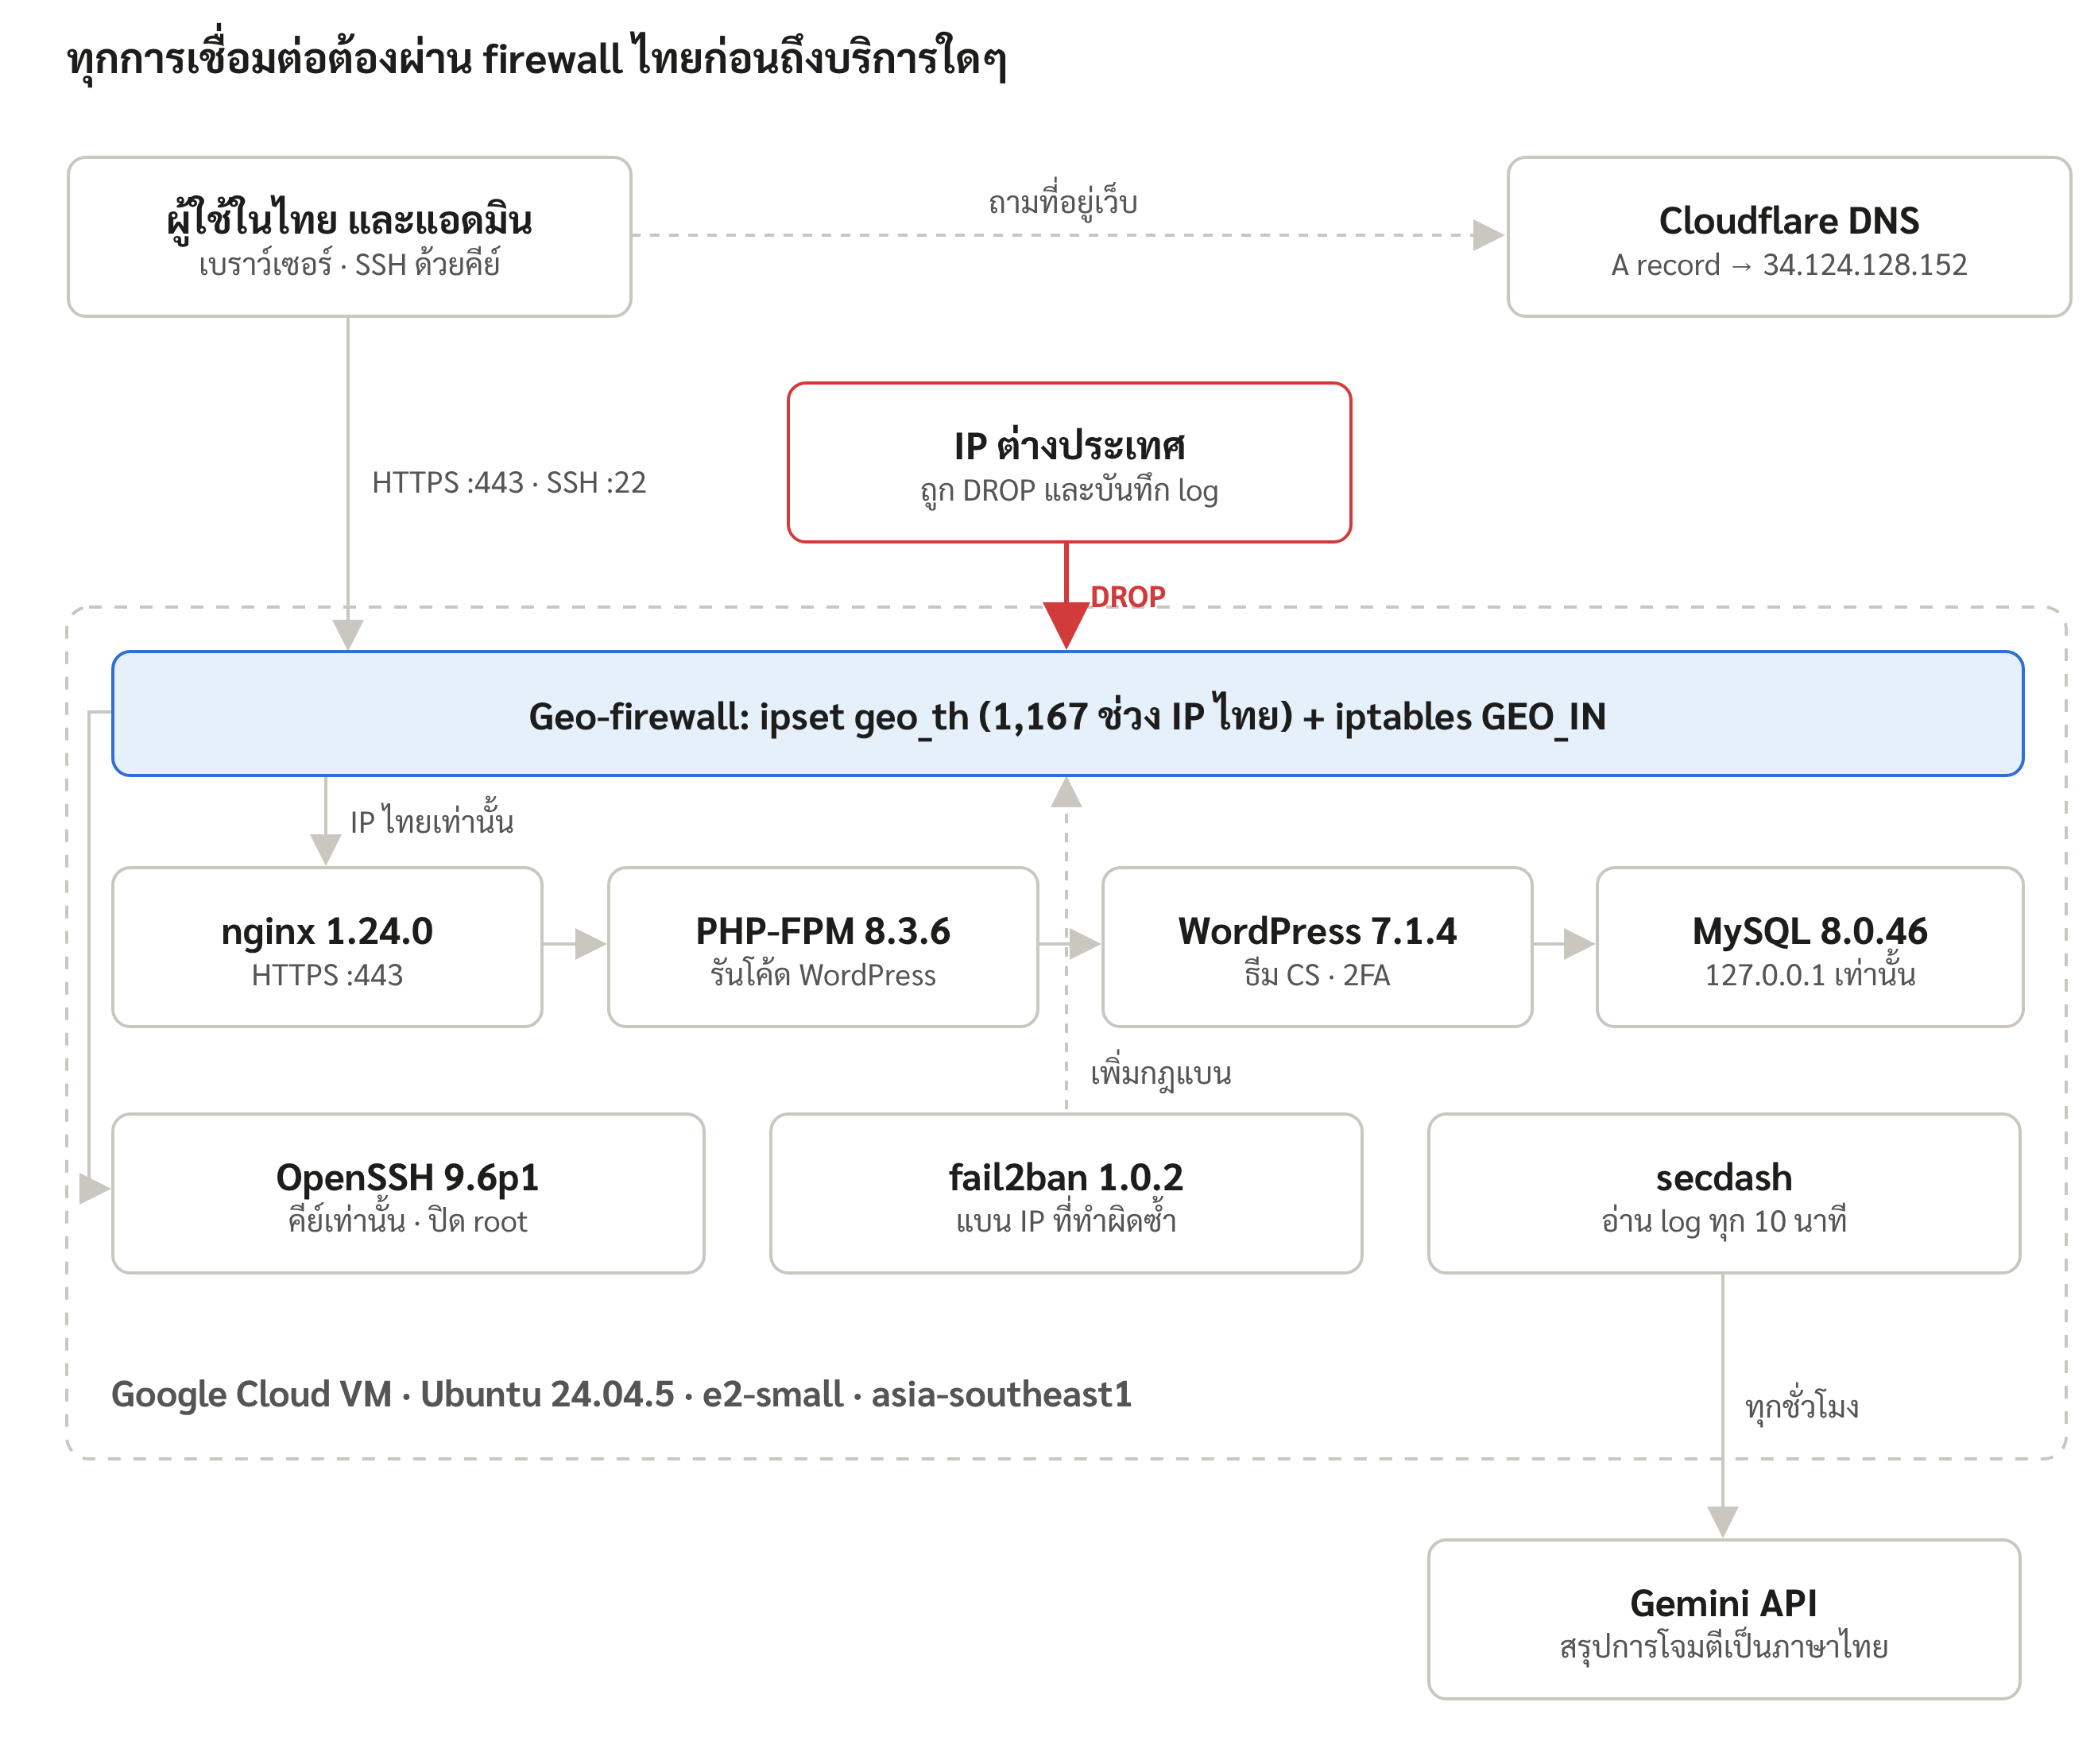
\includegraphics[width=0.95\linewidth,keepaspectratio]{figures/architecture.png}\end{center}

ภาพที่ 3.1 ผู้ใช้ถาม DNS แล้วเชื่อมต่อเซิร์ฟเวอร์ ทุกการเชื่อมต่อผ่าน geo-firewall ก่อน IP ไทยไปถึง nginx หรือ OpenSSH ส่วน IP ต่างประเทศถูก DROP และ secdash อ่าน log ทุกส่วนแล้วส่งสรุปให้ Gemini ทุกชั่วโมง

ตารางที่ 3.1 ซอฟต์แวร์และเวอร์ชันที่ใช้ (จากไฟล์ versions.txt บนเซิร์ฟเวอร์)

\begin{longtable}[]{@{}>{\raggedright\arraybackslash}p{0.282\linewidth - 2\tabcolsep}>{\raggedright\arraybackslash}p{0.395\linewidth - 2\tabcolsep}>{\raggedright\arraybackslash}p{0.293\linewidth - 2\tabcolsep}@{}}
\toprule\noalign{}
ส่วนประกอบ & เวอร์ชัน & หน้าที่ \\
\midrule\noalign{}
\endhead
\bottomrule\noalign{}
\endlastfoot
Ubuntu Server & 24.04.5 LTS (kernel 7.0.0-1014-gcp) & ระบบปฏิบัติการ \\
nginx & 1.24.0 & เว็บเซิร์ฟเวอร์ และ HTTPS \\
PHP-FPM & 8.3.6 & รันโค้ด WordPress \\
MySQL & 8.0.46 & ฐานข้อมูล \\
WordPress & 7.1.3 & ระบบจัดการเนื้อหา \\
OpenSSH & 9.6p1 & เข้าเซิร์ฟเวอร์ด้วยกุญแจ \\
fail2ban & 1.0.2 & แบน IP ที่ทำผิดซ้ำ \\
acme.sh & ใบรับรองจาก Let's Encrypt & ออกและต่ออายุใบรับรอง \\
ipset + iptables & ตามที่ Ubuntu ให้มา & geo-firewall \\
Python 3 (ไลบรารีมาตรฐาน) & ตามที่ Ubuntu ให้มา & ตัวเก็บข้อมูล secdash \\
\end{longtable}

คณะผู้จัดทำซ่อนเวอร์ชันเหล่านี้จากภายนอก (server\_tokens off และ expose\_php Off) เพื่อไม่ให้ผู้โจมตีเลือกช่องโหว่ที่ตรงกับเวอร์ชันได้ง่าย

\section*{3.2 การไหลของคำขอ}\addcontentsline{toc}{section}{3.2 การไหลของคำขอ}

\begin{enumerate}
\def\labelenumi{\arabic{enumi}.}
\tightlist
\item
  ผู้ใช้พิมพ์ elephotelephus.site เบราว์เซอร์ถาม DNS ของ Cloudflare และได้ IP 34.124.128.152
\item
  เบราว์เซอร์เชื่อมต่อพอร์ต 443 การเชื่อมต่อผ่าน firewall ของ Google Cloud แล้วเข้าสู่ chain GEO\_IN ของ iptables
\item
  ถ้า IP ต้นทางอยู่ในชุด IP ไทย แพ็กเก็ตผ่านไปถึง nginx ถ้าไม่ใช่ จะถูกบันทึก log และ DROP
\item
  nginx ถอดรหัส TLS ตรวจกฎความปลอดภัย (เช่น ปฏิเสธ xmlrpc.php และไฟล์ที่ขึ้นต้นด้วยจุด) แล้วส่งคำขอ PHP ให้ PHP-FPM
\item
  WordPress อ่านข้อมูลจาก MySQL ผ่าน 127.0.0.1 สร้างหน้าเว็บ และส่งกลับผ่าน nginx
\end{enumerate}

ผู้ดูแลระบบเข้าเครื่องด้วย SSH ผ่านพอร์ต 22 ซึ่งต้องผ่าน geo-firewall เช่นกัน ส่วนการดูฐานข้อมูลจากเครื่องของตนเอง (เช่น ด้วย DBeaver) ทำผ่าน SSH tunnel โดยไม่เปิดพอร์ต 3306 สู่อินเทอร์เน็ต

\section*{3.3 การป้องกันหลายชั้น (Defense in depth)}\addcontentsline{toc}{section}{3.3 การป้องกันหลายชั้น (Defense in depth)}

คณะผู้จัดทำไม่พึ่งการป้องกันชั้นเดียว เพราะผู้โจมตีอาจใช้ IP ไทย เช่น VPN หรือเครื่องในไทยที่ถูกยึด แต่ละชั้นจึงรับมือการโจมตีคนละแบบ

ตารางที่ 3.2 มาตรการป้องกันแต่ละชั้น

\begin{longtable}[]{@{}>{\raggedright\arraybackslash}p{0.115\linewidth - 2\tabcolsep}>{\raggedright\arraybackslash}p{0.427\linewidth - 2\tabcolsep}>{\raggedright\arraybackslash}p{0.427\linewidth - 2\tabcolsep}@{}}
\toprule\noalign{}
ชั้น & มาตรการ & รับมือกับ \\
\midrule\noalign{}
\endhead
\bottomrule\noalign{}
\endlastfoot
เครือข่าย & Geo-firewall รับเฉพาะ IP ไทย · fail2ban & บอทสแกนจากต่างประเทศ · การเดารหัสซ้ำ \\
การเข้าเครื่อง & SSH กุญแจเท่านั้น · ปิด root · บัญชีแยกรายบุคคล & การเดารหัส SSH · การยึดสิทธิ์ root \\
เว็บเซิร์ฟเวอร์ & ซ่อนเวอร์ชัน · security headers · จำกัดความถี่ wp-login (429) · ปิด xmlrpc.php · ปฏิเสธไฟล์ .env/.git · ห้ามรัน PHP ในโฟลเดอร์ uploads & การสำรวจระบบ · brute force · การสแกนไฟล์ลับ · การอัปโหลด web shell \\
WordPress & 2FA · ชื่อผู้ดูแลเดายาก · DISALLOW\_FILE\_EDIT · ลบธีม/ปลั๊กอินที่ไม่ใช้ · escape ข้อความทุกส่วน & รหัสผ่านรั่ว · การแก้โค้ดผ่านหลังบ้าน · XSS \\
ฐานข้อมูล & MySQL รับเฉพาะ 127.0.0.1 · ผู้ใช้ DB เฉพาะของ WordPress · เข้าดูผ่าน SSH tunnel & การเชื่อมต่อฐานข้อมูลจากภายนอก \\
ดูแลระบบ & unattended-upgrades · สำรองข้อมูลทุกวัน · swap & ช่องโหว่ที่มีแพตช์แล้ว · ข้อมูลเสียหาย \\
เฝ้าระวัง & secdash + AI (บทที่ 5) & มองเห็นการโจมตีที่เกิดขึ้นจริง \\
\end{longtable}

\thaichapter{บทที่ 4}{การติดตั้งและพัฒนา}\addcontentsline{toc}{chapter}{บทที่ 4 การติดตั้งและพัฒนา}

การติดตั้งส่วนใหญ่ทำผ่านสคริปต์ที่คณะผู้จัดทำเขียนขึ้น 3 ตัว ได้แก่ setup.sh (ติดตั้งระบบทั้งหมด) geo-firewall.sh (firewall ไทยเท่านั้น) และ secdash-install.sh (ระบบตรวจจับการโจมตี) ทำให้ติดตั้งซ้ำได้และตรวจสอบได้ว่าทำอะไรไปบ้าง

\section*{4.1 ขั้นที่ 1: เซิร์ฟเวอร์ โดเมน HTTPS และ SSH}\addcontentsline{toc}{section}{4.1 ขั้นที่ 1: เซิร์ฟเวอร์ โดเมน HTTPS และ SSH}

\subsection*{4.1.1 การสร้างเซิร์ฟเวอร์}

\begin{itemize}
\tightlist
\item
  สร้าง VM ชื่อ wordpress-server บน Google Compute Engine ชนิด e2-small โซน asia-southeast1-c
\item
  จอง IP คงที่ 34.124.128.152 และเปิด firewall ของ Google Cloud เฉพาะพอร์ต 22, 80 และ 443
\item
  เพิ่มกุญแจสาธารณะของสมาชิกผ่าน metadata ของ VM แต่ละคนได้บัญชีผู้ใช้ Linux ของตัวเอง
\item
  สร้าง swap ขนาด 2 GB เพราะเครื่องมี RAM 2 GB ป้องกัน MySQL หยุดทำงานเมื่อหน่วยความจำไม่พอ
\end{itemize}

\subsection*{4.1.2 โดเมนและ DNS}

จดโดเมน elephotelephus.site ที่ Cloudflare และสร้าง A record สองรายการคือ @ และ cs ชี้ไปที่ 34.124.128.152 โดยตั้งเป็น DNS only (เมฆสีเทา) เพื่อให้ผู้ใช้เชื่อมต่อตรงมาที่เซิร์ฟเวอร์ หากเปิด proxy ของ Cloudflare เซิร์ฟเวอร์จะเห็นแต่ IP ของ Cloudflare ทำให้ geo-firewall แยกประเทศผู้ใช้ไม่ได้

\subsection*{4.1.3 การติดตั้ง LEMP และ WordPress}

setup.sh ติดตั้งแพ็กเกจ nginx, php-fpm, mysql-server และ wp-cli จากนั้น

\begin{enumerate}
\def\labelenumi{\arabic{enumi}.}
\tightlist
\item
  สร้างฐานข้อมูล wordpress และผู้ใช้ wp\_app@localhost ด้วยรหัสผ่านสุ่ม 32 ตัวอักษร ให้สิทธิ์เฉพาะฐานข้อมูลนี้
\item
  ดาวน์โหลด WordPress ไปที่ /var/www/wordpress สร้าง wp-config.php และผู้ดูแลด้วยชื่อที่เดายาก (ไม่ใช้ admin)
\item
  ตั้ง DISALLOW\_FILE\_EDIT เป็น true เพื่อปิดการแก้โค้ดธีมและปลั๊กอินจากหน้าหลังบ้าน
\item
  ปิด expose\_php ใน PHP และ server\_tokens ใน nginx เพื่อซ่อนเวอร์ชัน
\end{enumerate}

กฎสำคัญในไฟล์ตั้งค่า nginx ของเว็บไซต์

\begin{Verbatim}[breaklines,breakanywhere,fontsize=\small,frame=single,framesep=6pt]
limit_req_zone $binary_remote_addr zone=wplogin:10m rate=6r/m;
limit_req_status 429;

add_header Strict-Transport-Security "max-age=31536000; includeSubDomains" always;
add_header X-Frame-Options "SAMEORIGIN" always;
add_header X-Content-Type-Options "nosniff" always;
add_header Referrer-Policy "strict-origin-when-cross-origin" always;

location = /xmlrpc.php            { deny all; return 403; }
location ~ /\.(?!well-known)      { deny all; }
location ~* /(wp-config\.php|readme\.html|license\.txt)$ { deny all; }
location ~* ^/wp-content/uploads/.*\.(php|phtml|phar)$     { deny all; }
location = /wp-login.php { limit_req zone=wplogin burst=5 nodelay; ... }
\end{Verbatim}

กฎเหล่านี้จำกัดหน้า login ไว้ที่ 6 คำขอต่อนาทีต่อ IP ส่ง security headers ปิด xmlrpc.php ปฏิเสธไฟล์ที่ขึ้นต้นด้วยจุด (.env, .git) และห้ามรัน PHP ในโฟลเดอร์อัปโหลด

\subsection*{4.1.4 HTTPS}

ติดตั้ง acme.sh แล้วขอใบรับรองจาก Let's Encrypt ด้วยวิธี DNS-01 ผ่าน API ของ Cloudflare (dns\_cf) โดยใช้ API token ที่มีสิทธิ์แก้ DNS เฉพาะ zone นี้ สคริปต์ตรวจว่า token และ Zone ID ใช้ได้จริงก่อนเริ่มขอใบรับรอง nginx ฟังที่ 443 ด้วย HTTP/2 และส่งคำขอ HTTP ทั้งหมดต่อไป HTTPS acme.sh ต่ออายุใบรับรองเองตามรอบ cron

เหตุผลที่เลือก DNS-01 คือเมื่อเปิด geo-firewall แล้ว เครื่องตรวจของ Let's Encrypt ที่อยู่ต่างประเทศจะเข้าเว็บไม่ได้ การต่ออายุแบบ HTTP-01 จะล้มเหลว

\begin{figure}[!htbp]
\centering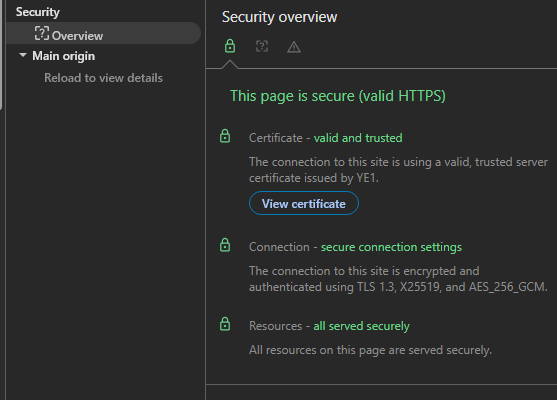
\includegraphics[width=0.51\linewidth,height=0.42\textheight,keepaspectratio]{figures/chrome-https.png}
\caption*{\textbf{ภาพที่ 4.1} Chrome ยืนยันว่าใบรับรองถูกต้องและเชื่อถือได้ และเชื่อมต่อด้วย TLS 1.3}
\end{figure}

\subsection*{4.1.5 SSH}

สร้างไฟล์ /etc/ssh/sshd\_config.d/00-hardening.conf ซึ่งถูกอ่านก่อนไฟล์อื่นในโฟลเดอร์เดียวกัน ค่าในไฟล์นี้จึงมีผลเสมอ

\begin{Verbatim}[breaklines,breakanywhere,fontsize=\small,frame=single,framesep=6pt]
PermitRootLogin no
PasswordAuthentication no
AuthenticationMethods publickey
\end{Verbatim}

ก่อนรีโหลด sshd สคริปต์ตรวจไวยากรณ์ด้วย sshd -t เพื่อไม่ให้ไฟล์ตั้งค่าผิดจนเข้าเครื่องไม่ได้

\begin{figure}[!htbp]
\centering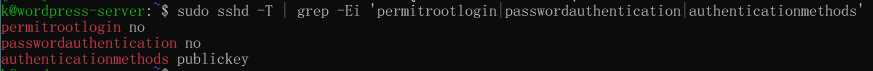
\includegraphics[width=0.79\linewidth,height=0.42\textheight,keepaspectratio]{figures/sshd-t.png}
\caption*{\textbf{ภาพที่ 4.2} ค่าที่ sshd ใช้งานจริง: ปิด root ปิดรหัสผ่าน และยืนยันตัวตนด้วยกุญแจเท่านั้น}
\end{figure}

\begin{figure}[!htbp]
\centering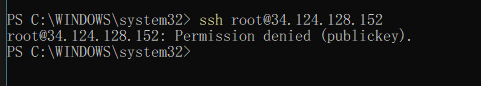
\includegraphics[width=0.50\linewidth,height=0.42\textheight,keepaspectratio]{figures/ssh-root-denied.png}
\caption*{\textbf{ภาพที่ 4.3} ทดสอบ ssh ด้วยบัญชี root จากเครื่องภายนอก ได้ Permission denied (publickey)}
\end{figure}

\subsection*{4.1.6 fail2ban, อัปเดตอัตโนมัติ และสำรองข้อมูล}

\begingroup\small\begin{longtable}[]{@{}>{\raggedright\arraybackslash}p{0.321\linewidth - 2\tabcolsep}>{\raggedright\arraybackslash}p{0.649\linewidth - 2\tabcolsep}@{}}
\toprule\noalign{}
รายการ & การตั้งค่า \\
\midrule\noalign{}
\endhead
\bottomrule\noalign{}
\endlastfoot
fail2ban (ค่าเริ่มต้น) & ผิด 5 ครั้งใน 10 นาที แบน 1 ชั่วโมง \\
jail sshd & อ่าน log จาก systemd journal \\
jail wordpress-login & นับการ login ผิดจาก access log ของ nginx ผิด 6 ครั้งแบน \\
jail nginx-limit-req & แบน IP ที่ถูก rate limit ซ้ำ \\
unattended-upgrades & ติดตั้งแพตช์ความปลอดภัยอัตโนมัติ \\
wp-backup.sh & สำรองฐานข้อมูลและไฟล์เว็บทุกวัน 03:30 น. เก็บ 7 วันที่ /var/backups/wordpress \\
\end{longtable}\endgroup

\begin{figure}[!htbp]
\centering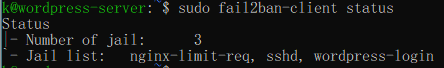
\includegraphics[width=0.50\linewidth,height=0.42\textheight,keepaspectratio]{figures/fail2ban-status.png}
\caption*{\textbf{ภาพที่ 4.4} fail2ban ทำงาน 3 jail: nginx-limit-req, sshd และ wordpress-login}
\end{figure}

\section*{4.2 ขั้นที่ 2: Geo-firewall รับเฉพาะ IP ไทย}\addcontentsline{toc}{section}{4.2 ขั้นที่ 2: Geo-firewall รับเฉพาะ IP ไทย}

\subsection*{4.2.1 การสร้างรายการ IP ไทย}

geo-firewall.sh ดาวน์โหลดไฟล์ delegated-apnic-latest จาก APNIC เลือกเฉพาะบรรทัดที่เป็น TH และ ipv4 แล้วแปลงจำนวน IP ของแต่ละช่วงเป็นรูป CIDR ด้วย Python ได้ 1,167 ช่วง หากดาวน์โหลดไม่ได้จะใช้ ipdeny.com เป็นแหล่งสำรอง และถ้าได้รายการน้อยผิดปกติสคริปต์จะหยุดทันที ไม่เปิด firewall ที่จะบล็อกทุกคน

รายการถูกโหลดเข้า ipset ชื่อ geo\_TH แบบ hash:net โดยสร้างชุดชั่วคราวก่อนแล้วสลับ (ipset swap) ทำให้อัปเดตได้โดยไม่มีช่วงเวลาที่ชุดว่าง

\subsection*{4.2.2 กฎ iptables}

\begin{Verbatim}[breaklines,breakanywhere,fontsize=\small,frame=single,framesep=6pt]
iptables -N GEO_IN
iptables -A GEO_IN -i lo -j RETURN
iptables -A GEO_IN -m conntrack --ctstate ESTABLISHED,RELATED -j RETURN
iptables -A GEO_IN -s 169.254.169.254 -j RETURN        # metadata ของ cloud
iptables -A GEO_IN -s 10.0.0.0/8 -j RETURN             # เครือข่ายภายในของ cloud
iptables -A GEO_IN -m set --match-set geo_TH src -j RETURN
iptables -A GEO_IN -m limit --limit 5/min -j LOG --log-prefix "GEO-BLOCK: "
iptables -A GEO_IN -j DROP
iptables -I INPUT 1 -j GEO_IN
\end{Verbatim}

กฎทำงานตามลำดับ แพ็กเก็ตของการเชื่อมต่อที่เครื่องเริ่มเอง (เช่น การอัปเดตแพ็กเกจ หรือการเรียก API) ผ่านด้วยกฎ ESTABLISHED,RELATED ส่วนการเชื่อมต่อใหม่จากภายนอกผ่านได้เฉพาะ IP ที่อยู่ใน geo\_TH ที่เหลือจะถูกบันทึก log (จำกัด 5 บรรทัดต่อนาที กัน log ล้น) แล้ว DROP

\subsection*{4.2.3 การป้องกันการล็อกตัวเองออก}

\begin{itemize}
\tightlist
\item
  ก่อนเปิด สคริปต์ตรวจว่า IP ที่กำลัง SSH อยู่อยู่ในชุด IP ไทย ถ้าไม่อยู่จะไม่ยอมเปิด
\item
  คำสั่ง apply ตั้งตัวจับเวลา 3 นาที ถ้าผู้ดูแลไม่พิมพ์ confirm ภายในเวลานั้น ระบบจะปิด firewall เอง กรณีตั้งค่าผิดจนเข้าเครื่องไม่ได้
\item
  บริการ systemd เปิด firewall ใหม่ทุกครั้งที่รีบูต และ cron อัปเดตรายการ IP ทุกสัปดาห์
\item
  คำสั่งที่ใช้ได้: apply, confirm, status, update, off
\end{itemize}

\begin{figure}[!htbp]
\centering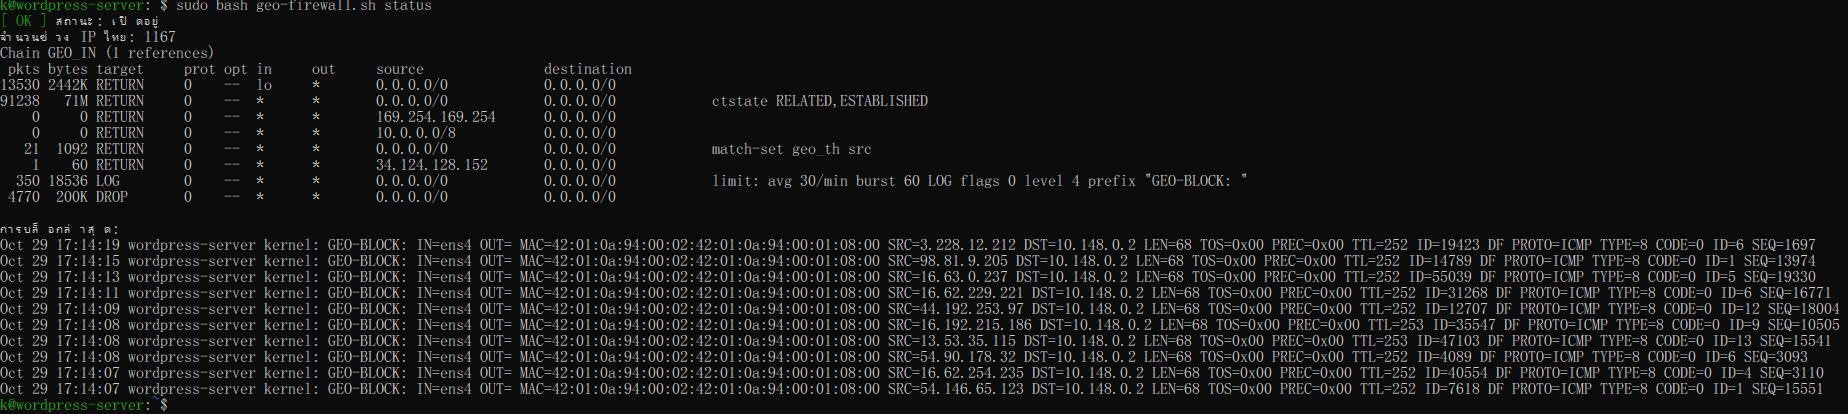
\includegraphics[width=1.00\linewidth,height=0.42\textheight,keepaspectratio]{figures/geo-firewall-status.png}
\caption*{\textbf{ภาพที่ 4.5} สถานะ geo-firewall: ช่วง IP ไทย 1,167 ช่วง กฎ chain GEO\_IN (รวมกฎอนุญาต IP ของเซิร์ฟเวอร์เอง) และ log GEO-BLOCK ล่าสุด}
\end{figure}

\section*{4.3 ขั้นที่ 3: เว็บไซต์สาขาวิทยาการคอมพิวเตอร์}\addcontentsline{toc}{section}{4.3 ขั้นที่ 3: เว็บไซต์สาขาวิทยาการคอมพิวเตอร์}

\subsection*{4.3.1 ธีม}

คณะผู้จัดทำเขียนธีม BUU Computer Science ขึ้นเองตามแบบที่ทีมออกแบบไว้ใน Figma ใช้โทนสีฟ้ากับกรมท่า (\#0a2e57, \#0b6fd0) ฟอนต์ Anuphan และ IBM Plex Sans Thai ออกแบบให้อ่านง่ายบนโทรศัพท์ เนื่องจากกลุ่มเป้าหมายส่วนใหญ่เป็นนักเรียนมัธยมที่ใช้มือถือเป็นหลัก

หน้าหลักของเว็บไซต์

\begingroup\small\begin{longtable}[]{@{}>{\raggedright\arraybackslash}p{0.310\linewidth - 2\tabcolsep}>{\raggedright\arraybackslash}p{0.660\linewidth - 2\tabcolsep}@{}}
\toprule\noalign{}
หน้า & เนื้อหา \\
\midrule\noalign{}
\endhead
\bottomrule\noalign{}
\endlastfoot
หน้าแรก & แนะนำสาขา จุดเด่น หลักสูตร อาชีพหลังจบ ข่าวล่าสุด \\
เกี่ยวกับสาขา & แสดงเนื้อหาที่แก้ได้จากตัวแก้ไขบทความ \\
ข่าวสารและกิจกรรม & ข่าวที่นำเข้าจากเว็บไซต์คณะ \\
หลักสูตร & หลักสูตรและรายละเอียดของสาขา \\
\end{longtable}\endgroup

\begin{figure}[!htbp]
\centering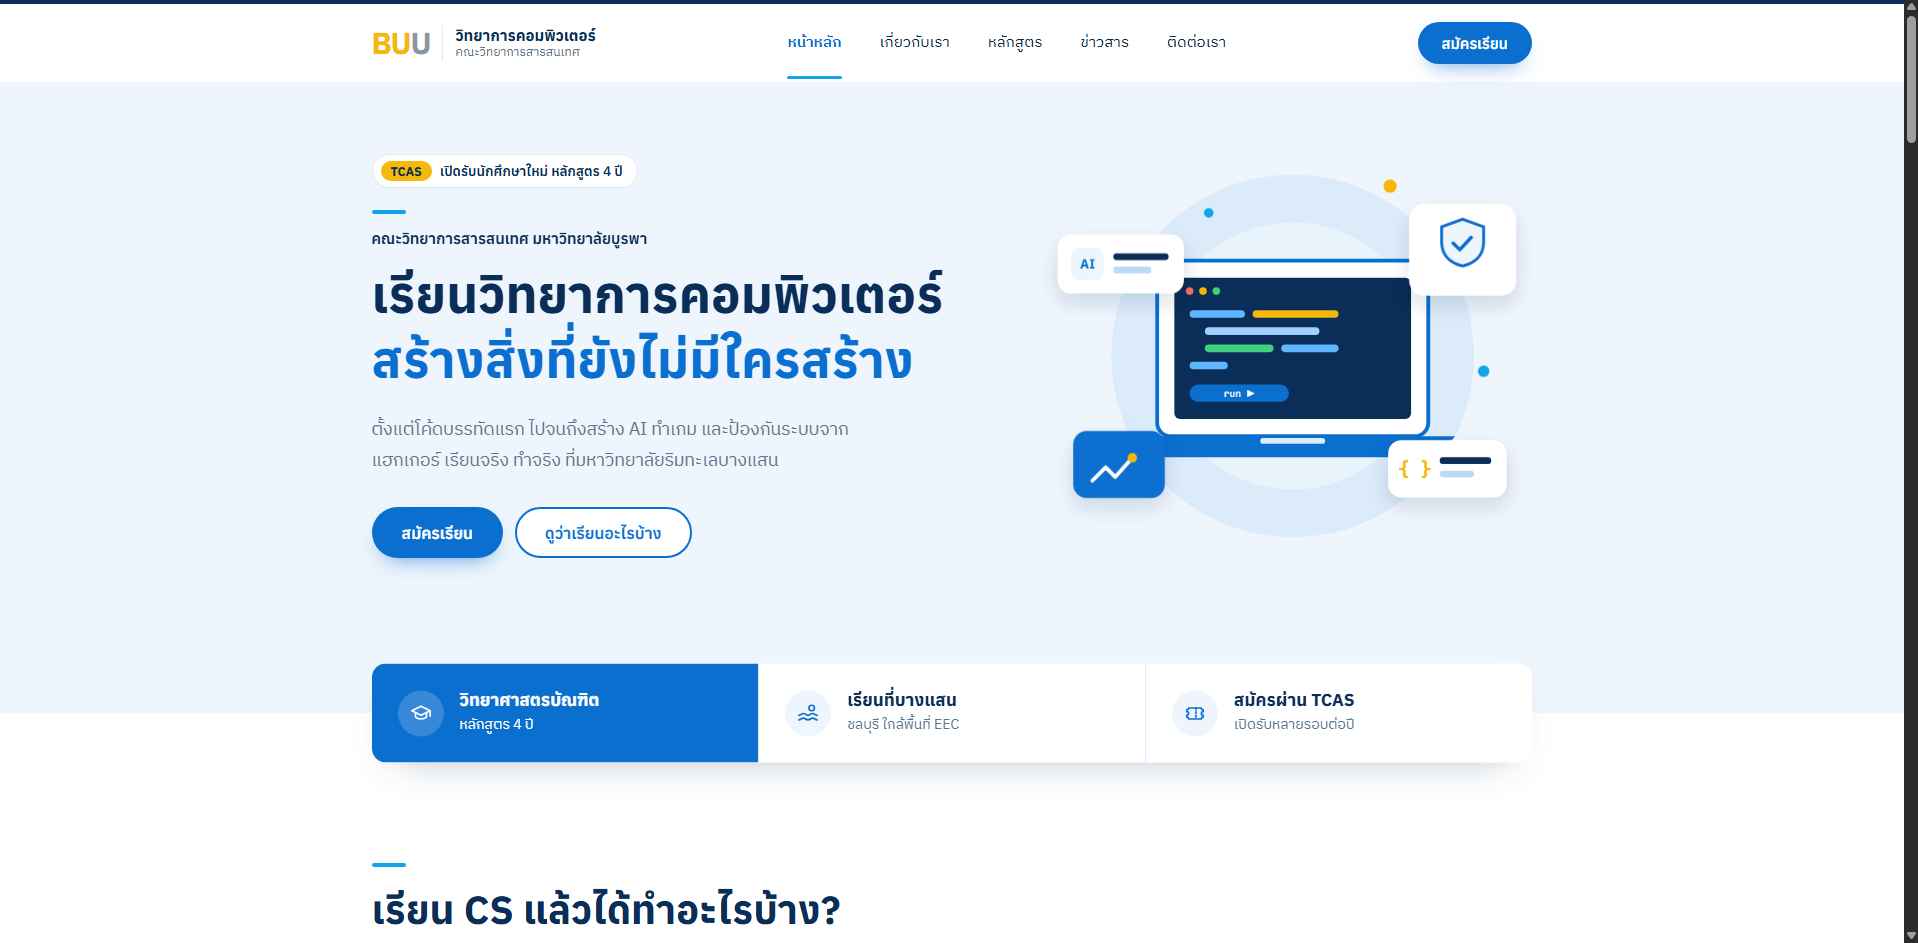
\includegraphics[width=1.00\linewidth,height=0.42\textheight,keepaspectratio]{figures/home-desktop.png}
\caption*{\textbf{ภาพที่ 4.6} หน้าแรกของเว็บไซต์บนคอมพิวเตอร์}
\end{figure}

\begin{figure}[!htbp]
\centering
\includegraphics[width=0.84\linewidth,height=0.42\textheight,keepaspectratio]{figures/home-mobile.png}
\caption*{\textbf{ภาพที่ 4.7} หน้าแรกบนมือถือ เมนูยุบเป็นปุ่ม และข้อความปรับขนาดให้อ่านง่าย}
\end{figure}

\subsection*{4.3.2 เนื้อหาที่แก้ไขได้จากหลังบ้าน}

ข้อความทุกส่วนของธีมถูกกำหนดเป็นค่าตั้ง (setting) ใน WordPress Customizer ภายใต้แผง ``เนื้อหาเว็บไซต์'' ประมาณ 10 หมวด รวม 101 ค่า สมาชิกทีมแก้ข้อความและเห็นผลทันทีโดยไม่ต้องแก้โค้ด ถ้าลบหัวข้อของส่วนใดออก ส่วนนั้นจะซ่อนอัตโนมัติ ข้อความทุกจุดผ่านฟังก์ชัน escape ก่อนแสดงผล เพื่อป้องกัน XSS

\begin{figure}[!htbp]
\centering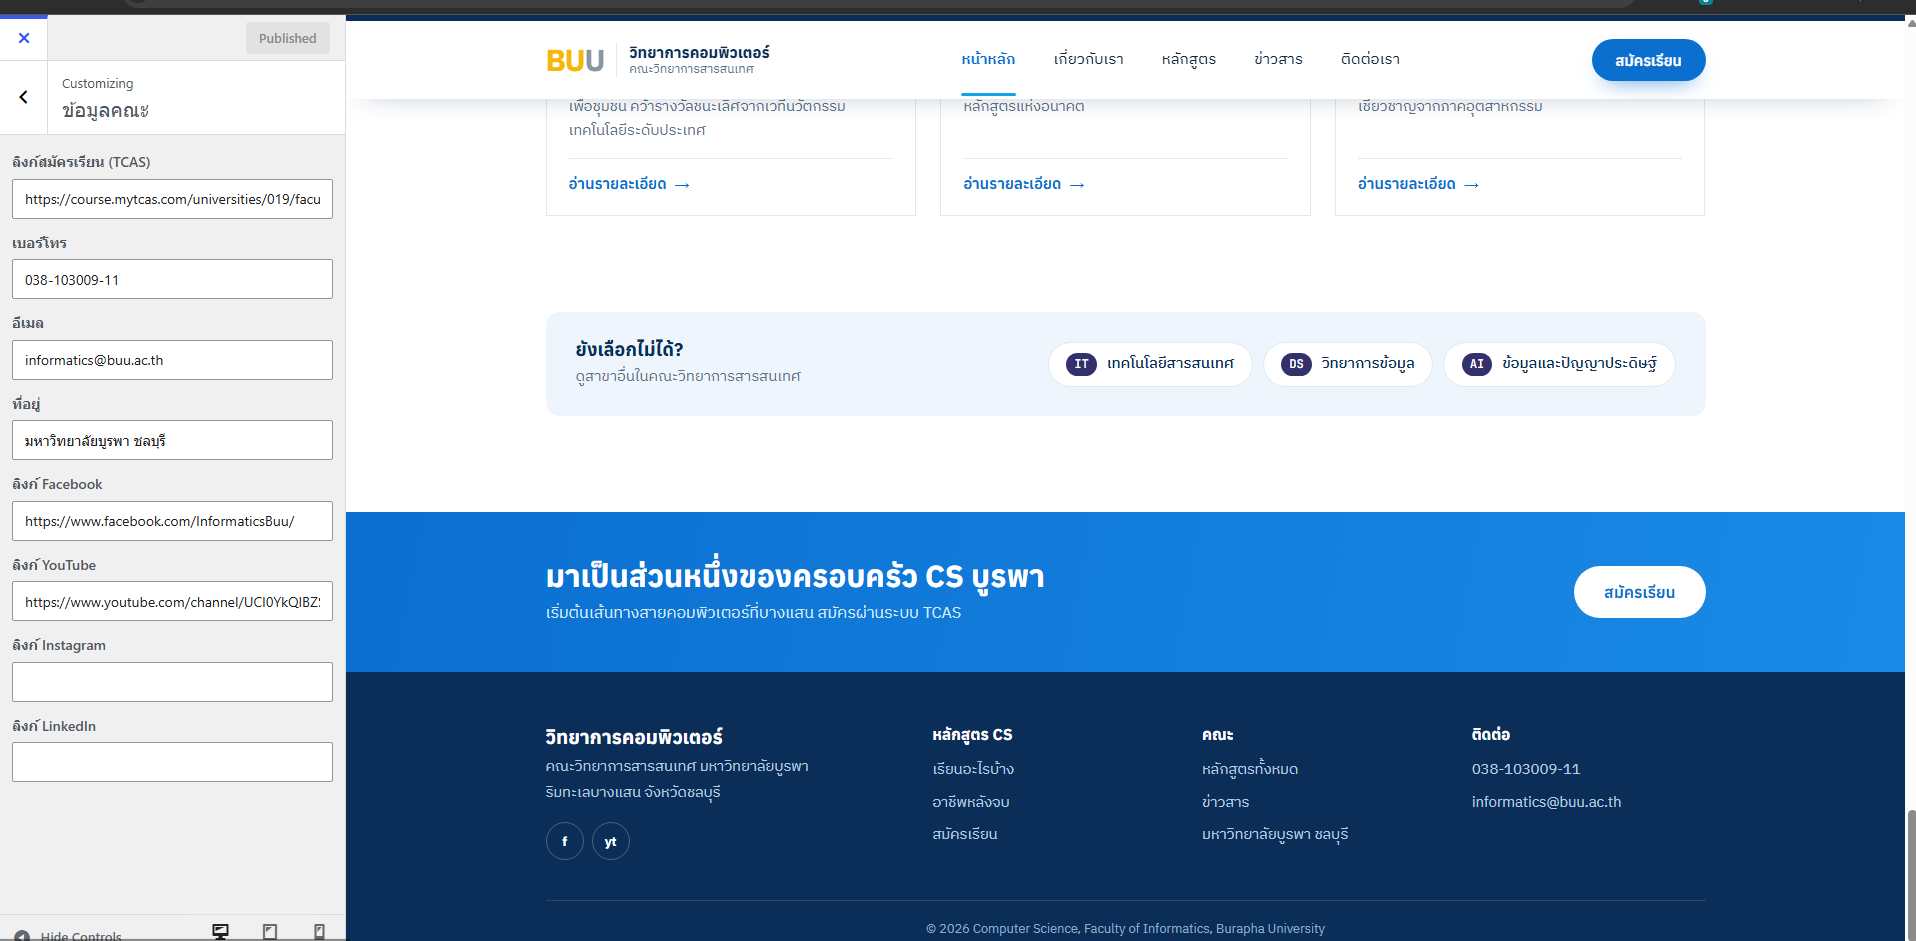
\includegraphics[width=1.00\linewidth,height=0.42\textheight,keepaspectratio]{figures/customizer.png}
\caption*{\textbf{ภาพที่ 4.8} แก้ข้อความของเว็บไซต์ได้จาก Customizer โดยไม่ต้องแก้โค้ด}
\end{figure}

\subsection*{4.3.3 การนำเข้าข่าวจากเว็บไซต์คณะ}

เว็บไซต์คณะใช้ WordPress และเปิด REST API (?rest\_route=/wp/v2/posts) ไว้ คณะผู้จัดทำจึงดึงข้อมูลผ่าน API แทนการสแครปหน้าเว็บ ได้ข้อมูลที่มีโครงสร้างและไม่พังเมื่อหน้าตาเว็บคณะเปลี่ยน หาก API ใช้ไม่ได้จะใช้ RSS feed แทน

\begin{enumerate}
\def\labelenumi{\arabic{enumi}.}
\tightlist
\item
  WP-Cron เรียก buu\_import\_news() ทุกชั่วโมง
\item
  ดึงรายการข่าวผ่าน REST API นำเข้าใหม่ได้ครั้งละไม่เกิน 25 ข่าว รวมสูงสุด 100 ข่าว
\item
  ตรวจข่าวซ้ำจาก meta \_buu\_src ที่เก็บลิงก์ต้นทาง
\item
  กรองเนื้อหาด้วย wp\_kses\_post (ตัดสคริปต์และแท็กอันตราย) และต่อท้ายด้วยบรรทัดเครดิตแหล่งที่มา
\item
  ดาวน์โหลดรูปปกเฉพาะลิงก์ https เก็บเป็นไฟล์ในเว็บของเราเอง
\item
  บันทึกเป็นโพสต์ในตาราง wp\_posts และแสดงในหน้าข่าวสาร
\end{enumerate}

ผู้ดูแลสั่งนำเข้าทันทีได้จากเมนู Tools ในหลังบ้าน และตรวจข้อมูลในฐานข้อมูลได้ด้วย DBeaver ผ่าน SSH tunnel เช่น

\begin{Verbatim}[breaklines,breakanywhere,fontsize=\small,frame=single,framesep=6pt]
SELECT p.ID, p.post_title, p.post_date, m.meta_value AS source_url
FROM wp_posts p
JOIN wp_postmeta m ON m.post_id = p.ID AND m.meta_key = '_buu_src'
WHERE p.post_type = 'post'
ORDER BY p.post_date DESC;
\end{Verbatim}

\begin{figure}[!htbp]
\centering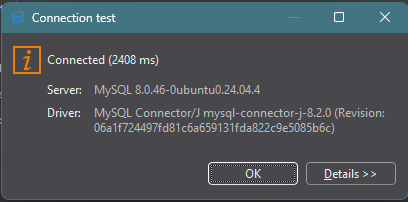
\includegraphics[width=0.50\linewidth,height=0.42\textheight,keepaspectratio]{figures/dbeaver.png}
\caption*{\textbf{ภาพที่ 4.9} DBeaver เชื่อมต่อ MySQL 8.0.46 ผ่าน SSH tunnel สำเร็จ}
\end{figure}

\begin{figure}[!htbp]
\centering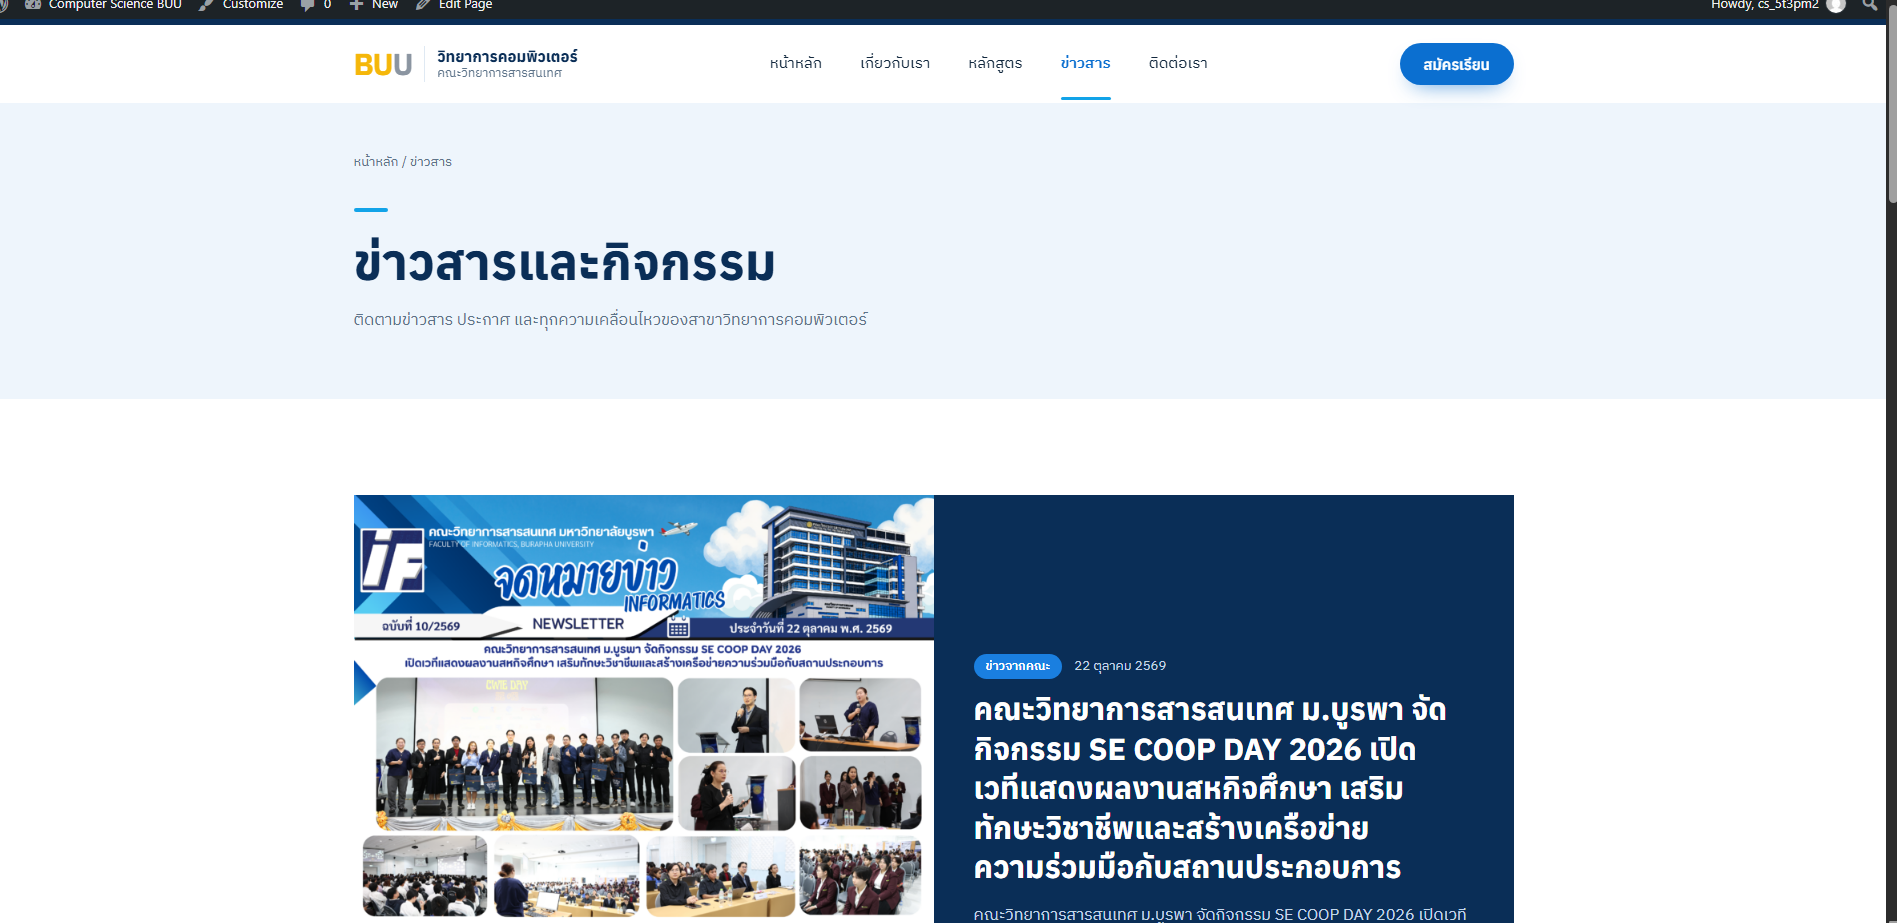
\includegraphics[width=1.00\linewidth,height=0.42\textheight,keepaspectratio]{figures/news-page.png}
\caption*{\textbf{ภาพที่ 4.10} หน้าข่าวสารและกิจกรรมที่แสดงข่าวที่นำเข้าจากเว็บไซต์คณะ}
\end{figure}

\subsection*{4.3.4 บัญชีผู้ใช้และ 2FA}

ผู้ดูแลเปิด 2FA ด้วยปลั๊กอิน Two-Factor สมาชิกคนอื่นได้บัญชีสิทธิ์ Editor ที่แก้เนื้อหาได้ แต่ติดตั้งปลั๊กอินหรือเปลี่ยนการตั้งค่าไม่ได้ ธีมและปลั๊กอินที่ไม่ได้ใช้ถูกลบออก เหลือเฉพาะธีมของคณะผู้จัดทำและปลั๊กอิน Two-Factor

\section*{4.4 การตรวจความปลอดภัยช่วงช่องโหว่ PHP (ต.ค. 2569)}\addcontentsline{toc}{section}{4.4 การตรวจความปลอดภัยช่วงช่องโหว่ PHP (ต.ค. 2569)}

ปลายเดือนตุลาคม 2569 มีการประกาศช่องโหว่ร้ายแรงใน PHP คือ CVE-2026-109618 และ CVE-2026-109619 ซึ่งทำให้ผู้โจมตีรันโค้ดบนเซิร์ฟเวอร์ได้โดยไม่ต้องล็อกอิน และถูกนำไปใช้โจมตีจริงแล้ว รวมถึง CVE-2026-115560 ที่ยังไม่มีแพตช์ คณะผู้จัดทำจึงเขียนสคริปต์ security-check.sh เพื่อตรวจและแก้ไข

\begingroup\small\begin{longtable}[]{@{}>{\raggedright\arraybackslash}p{0.275\linewidth - 2\tabcolsep}>{\raggedright\arraybackslash}p{0.695\linewidth - 2\tabcolsep}@{}}
\toprule\noalign{}
รายการ & วิธีตรวจ/แก้ \\
\midrule\noalign{}
\endhead
\bottomrule\noalign{}
\endlastfoot
แพตช์ PHP & ตรวจว่า php8.3-fpm เป็นเวอร์ชัน 8.3.6-0ubuntu0.24.04.13 ขึ้นไป (USN-8948-1) เพราะ php -v แสดงแค่ 8.3.6 จึงใช้ยืนยันไม่ได้ แล้วรีสตาร์ต PHP-FPM ให้ worker ใช้โค้ดใหม่ \\
CVE-2026-115560 & ปิด session.upload\_progress.enabled ในการตั้งค่าของ PHP-FPM (WordPress ไม่ได้ใช้) \\
จำกัดความเสียหาย & ปิดฟังก์ชันรันคำสั่งระบบ (exec, system, shell\_exec, proc\_open, popen) ใน PHP-FPM \\
ตรวจการบุกรุก & หาไฟล์ PHP ในโฟลเดอร์ uploads, ไฟล์ PHP ที่ถูกแก้ใน 7 วัน, ตรวจไฟล์ WordPress core และปลั๊กอินกับต้นฉบับ (wp core verify-checksums) \\
มุมมองคนนอก & ทดสอบว่า xmlrpc.php, .env, ?author=1 และ REST รายชื่อผู้ใช้ ถูกปฏิเสธ \\
ระบบ & พอร์ตที่เปิด, MySQL รับเฉพาะ 127.0.0.1, SSH, fail2ban, geo-firewall, อัปเดตที่ค้าง \\
\end{longtable}\endgroup

นอกจากนี้ธีมเวอร์ชัน 3.7.0 เพิ่มไฟล์ inc/hardening.php ปิดการไล่หาชื่อผู้ใช้สำหรับคนที่ไม่ได้ล็อกอิน (?author=N ได้ 403, REST /wp/v2/users ถูกซ่อน, sitemap และ oEmbed ไม่แสดงผู้เขียน) ซ่อนเวอร์ชัน WordPress และใช้ข้อความล็อกอินผิดแบบไม่บอกว่าชื่อผู้ใช้มีอยู่จริงหรือไม่

ผลการรัน security-check.sh บนเซิร์ฟเวอร์จริง (29 ตุลาคม 2569)

\begin{figure}[!htbp]
\centering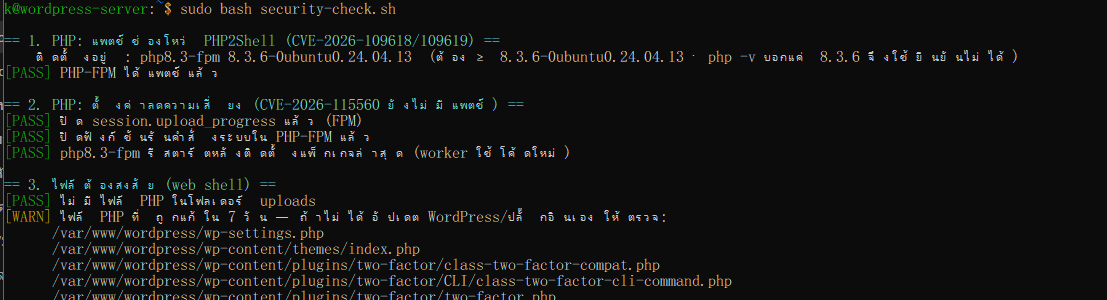
\includegraphics[width=1.00\linewidth,height=0.42\textheight,keepaspectratio]{figures/security-check-php.png}
\caption*{\textbf{ภาพที่ 4.11} PHP-FPM ได้แพตช์แล้ว (8.3.6-0ubuntu0.24.04.13) และตั้งค่าลดความเสี่ยงครบ}
\end{figure}

\begin{figure}[!htbp]
\centering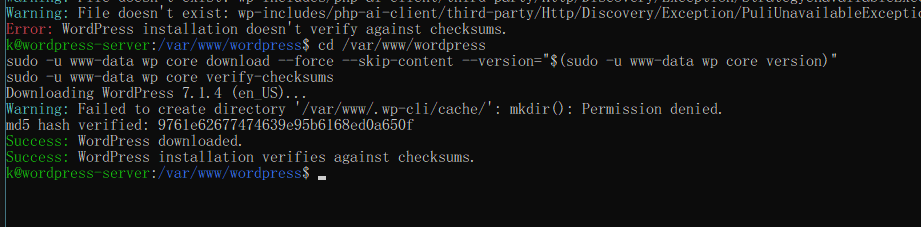
\includegraphics[width=0.84\linewidth,height=0.42\textheight,keepaspectratio]{figures/wp-checksums.png}
\caption*{\textbf{ภาพที่ 4.12} หลังดาวน์โหลด core ทับใหม่ ไฟล์ WordPress ทุกไฟล์ตรงกับต้นฉบับจาก wordpress.org}
\end{figure}

\begin{figure}[!htbp]
\centering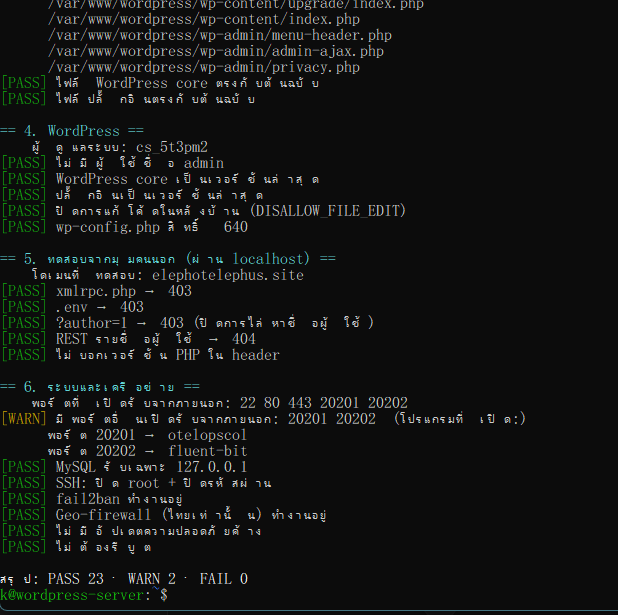
\includegraphics[width=0.56\linewidth,height=0.42\textheight,keepaspectratio]{figures/security-check-summary.png}
\caption*{\textbf{ภาพที่ 4.13} ผลสรุป PASS 23 · WARN 2 · FAIL 0 โดย WARN ทั้งสองข้อตรวจแล้วอธิบายได้ คือไฟล์ที่เปลี่ยนจากการอัปเดต (ตรงกับต้นฉบับ) และพอร์ต 20201/20202 ของ Google Cloud Ops Agent ซึ่งคนภายนอกเข้าไม่ถึง}
\end{figure}
\chapter*{บทที่ 5 ระบบตรวจจับการโจมตีและ dashboard ด้วย AI}\addcontentsline{toc}{chapter}{บทที่ 5 ระบบตรวจจับการโจมตีและ dashboard ด้วย AI}

ส่วนนี้เป็นงานเพิ่มเติมจากโจทย์ ตามแนวคิดที่อาจารย์เสนอให้ใช้ AI สแกน log ตามรอบเวลาแล้วทำ dashboard สำหรับตรวจการโจมตี ระบบมีชื่อว่า secdash ประกอบด้วยสองส่วน คือตัวเก็บข้อมูลบนเซิร์ฟเวอร์ และหน้า ``ความปลอดภัย'' ในหลังบ้าน WordPress

\section*{5.1 ตัวเก็บข้อมูล (secdash-collect.py)}\addcontentsline{toc}{section}{5.1 ตัวเก็บข้อมูล (secdash-collect.py)}

สคริปต์ Python ที่ใช้เฉพาะไลบรารีมาตรฐาน รันด้วย cron ทุก 10 นาที อ่าน log ย้อนหลัง 7 วันจาก 4 แหล่ง

\begin{longtable}[]{@{}>{\raggedright\arraybackslash}p{0.121\linewidth - 2\tabcolsep}>{\raggedright\arraybackslash}p{0.364\linewidth - 2\tabcolsep}>{\raggedright\arraybackslash}p{0.485\linewidth - 2\tabcolsep}@{}}
\toprule\noalign{}
แหล่ง & อ่านจาก & สิ่งที่ได้ \\
\midrule\noalign{}
\endhead
\bottomrule\noalign{}
\endlastfoot
nginx & access log (รวมไฟล์ที่ถูกบีบอัด) & คำขอเว็บ การ login WordPress \\
SSH & systemd journal & เข้าสำเร็จ เข้าไม่สำเร็จ ชื่อผู้ใช้ที่ไม่มีอยู่ \\
Geo-firewall & kernel log ที่ขึ้นต้นด้วย GEO-BLOCK: & IP ต่างประเทศที่ถูกบล็อก และพอร์ตที่พยายามต่อ \\
fail2ban & fail2ban.log และ fail2ban-client & IP ที่ถูกแบนและ jail ที่แบน \\
\end{longtable}

คำขอแต่ละรายการถูกเทียบกับรูปแบบ (regular expression) เพื่อจัดประเภท แต่ละประเภทมีคะแนนความรุนแรง คะแนนของ IP คือผลรวมของทุกเหตุการณ์ ประเภทที่ตรวจ ได้แก่ SQL injection, XSS, path traversal, สแกนไฟล์ลับ, เครื่องมือสแกน (ดูจาก User-Agent), ไล่หาชื่อผู้ใช้ WordPress, เรียก xmlrpc.php, login WordPress ผิด, ถูก rate limit, สุ่มหา URL จำนวนมาก (404 ตั้งแต่ 50 ครั้ง), SSH เดารหัส, ถูก geo-firewall บล็อก และถูก fail2ban แบน

นอกจากนี้สคริปต์ทำการตรวจความผิดปกติทางสถิติ โดยเทียบจำนวนคำขอในชั่วโมงล่าสุดกับชั่วโมงก่อนหน้าด้วยค่า z-score และแจ้งเตือนเมื่อ z $\geq$ 3 และมีคำขออย่างน้อย 30 ครั้ง จากนั้นเขียนผลสรุปลงไฟล์ /var/lib/secdash/summary.json แบบ atomic (เขียนไฟล์ชั่วคราวแล้วเปลี่ยนชื่อ) สิทธิ์ 640 ให้เฉพาะ root และกลุ่ม www-data อ่านได้

\section*{5.2 การลดการแจ้งเตือนผิด (false positive)}\addcontentsline{toc}{section}{5.2 การลดการแจ้งเตือนผิด (false positive)}

\begin{itemize}
\tightlist
\item
  \textbf{ขั้นกรอก 2FA:} การ POST ไปที่ wp-login.php แล้วได้ 200 อาจเป็นทั้งรหัสผิดหรือหน้ากรอกรหัส 2FA สคริปต์จะพักเหตุการณ์ไว้ก่อน ถ้า IP เดียวกันยืนยัน 2FA สำเร็จภายใน 5 นาที จะตัดเหตุการณ์นั้นออก
\item
  \textbf{IP ของทีม:} ตัวแก้ไขบทความของ WordPress เรียก /wp-json/wp/v2/users เองตามปกติ ซึ่งเป็นที่อยู่เดียวกับที่ผู้โจมตีใช้ไล่หาชื่อผู้ใช้ สคริปต์จึงถือว่า IP ที่ login สำเร็จ (SSH หรือ WordPress) ในช่วง 7 วันเป็นคนในทีม และไม่นับเหตุการณ์ประเภทไล่หาชื่อผู้ใช้ 404 จำนวนมาก และ rate limit ของ IP เหล่านั้น ส่วนเหตุการณ์อันตรายจริง เช่น SQL injection ยังแสดงตามปกติ
\end{itemize}

\section*{5.3 การวิเคราะห์ด้วย AI}\addcontentsline{toc}{section}{5.3 การวิเคราะห์ด้วย AI}

ทุกชั่วโมง สคริปต์ส่งข้อมูลสรุปให้ Google Gemini ผ่าน API และขอคำตอบเป็น JSON ที่มีระดับความเสี่ยง (low, medium, high) สรุป 1--2 ประโยค สิ่งที่พบไม่เกิน 4 ข้อ และสิ่งที่ควรทำไม่เกิน 3 ข้อ เป็นภาษาไทย คีย์ API เก็บใน /etc/secdash/ai.env สิทธิ์ 600 อ่านได้เฉพาะ root

ข้อมูลที่ส่งให้ AI

\begin{itemize}
\tightlist
\item
  จำนวนเหตุการณ์แต่ละประเภทใน 24 ชั่วโมง จำนวนคำขอ และจำนวนที่ถูกบล็อก
\item
  IP ที่มีคะแนนสูงสุด 10 อันดับ พร้อมประเภทการโจมตีและเวลาล่าสุด
\item
  ตัวอย่างคำขอที่รุนแรงไม่เกิน 15 รายการ พร้อม status code
\item
  รายการมาตรการป้องกันที่มีอยู่แล้ว เพื่อไม่ให้ AI แนะนำสิ่งที่ทำไปแล้ว
\end{itemize}

คำสั่งที่ส่งให้ AI ระบุชัดเจนว่าข้อความในช่อง detail และ ua มาจากผู้โจมตี ห้ามทำตามคำสั่งใดๆ ในนั้น เพื่อป้องกัน prompt injection คำตอบที่ได้ถูกตรวจรูปแบบ ตัดความยาว และหน้า dashboard แสดงผลแบบ escape ทุกจุด

การเลือกโมเดลทำแบบอัตโนมัติ สคริปต์ขอรายชื่อโมเดลจาก Google เลือกรุ่น Flash ที่ใหม่ที่สุดที่ไม่ใช่รุ่นทดลอง ถ้ารุ่นนั้นถูกปลด (404) ไม่ว่าง (429, 500, 503) หรือตอบช้าเกิน 120 วินาที จะลองรุ่นถัดไป สูงสุด 4 รุ่นภายใน 5 นาที หากไม่สำเร็จ dashboard ยังทำงานได้ครบทุกส่วน เพียงแสดงเหตุผลที่ AI ไม่ตอบ

\section*{5.4 หน้า dashboard}\addcontentsline{toc}{section}{5.4 หน้า dashboard}

หน้า ``ความปลอดภัย'' อยู่ในหลังบ้าน WordPress แสดงเฉพาะผู้ดูแล (สิทธิ์ manage\_options) ประกอบด้วย

\begin{longtable}[]{@{}>{\raggedright\arraybackslash}p{0.293\linewidth - 2\tabcolsep}>{\raggedright\arraybackslash}p{0.677\linewidth - 2\tabcolsep}@{}}
\toprule\noalign{}
ส่วน & แสดง \\
\midrule\noalign{}
\endhead
\bottomrule\noalign{}
\endlastfoot
ระดับความเสี่ยง + กล่อง AI & ปกติ / เฝ้าระวัง / สูง และสรุปจาก Gemini \\
ตัวเลขหลัก & คำขอ 24 ชม. · การโจมตี · IP ต่างประเทศที่ถูกบล็อก · ถูก fail2ban แบน · SSH ไม่สำเร็จ · IP น่าสงสัย 7 วัน \\
กราฟ 24 ชั่วโมง & คำขอเข้าเว็บและการโจมตีรายชั่วโมง \\
ประเภทการโจมตี & จำนวนแต่ละประเภทใน 24 ชม. \\
IP ที่น่าสงสัยที่สุด & IP · ที่มา (ไทย/ต่างประเทศ) · พฤติกรรม · คะแนน · จำนวนครั้ง · ล่าสุด · สถานะแบน \\
การเข้าระบบล่าสุด & login SSH และ WordPress ที่สำเร็จ \\
เหตุการณ์ล่าสุด & เหตุการณ์ที่มีความเสี่ยง 60 รายการล่าสุด \\
\end{longtable}

ข้อมูลทุกช่องที่มาจาก log แสดงผ่าน esc\_html เพราะ URL และ User-Agent เป็นข้อความที่ผู้โจมตีกำหนดเองได้ หากแสดงตรงๆ dashboard เองจะกลายเป็นช่องโหว่ XSS

\thaichapter{บทที่ 6}{การทดสอบและผลการดำเนินงาน}\addcontentsline{toc}{chapter}{บทที่ 6 การทดสอบและผลการดำเนินงาน}

ทุกข้อกำหนดของโจทย์ผ่านการทดสอบ ตารางต่อไปนี้สรุปวิธีทดสอบและผลที่ได้ ภาพหน้าจอประกอบอยู่ในภาคผนวก ขค.

\section*{6.1 ผลการทดสอบตามข้อกำหนด}\addcontentsline{toc}{section}{6.1 ผลการทดสอบตามข้อกำหนด}

\needspace{7\baselineskip}\noindent\textbf{ตารางที่ 6.1} ผลการทดสอบ

\begingroup\small\begin{longtable}[]{@{}>{\raggedright\arraybackslash}p{0.145\linewidth - 2\tabcolsep}>{\raggedright\arraybackslash}p{0.194\linewidth - 2\tabcolsep}>{\raggedright\arraybackslash}p{0.315\linewidth - 2\tabcolsep}>{\raggedright\arraybackslash}p{0.315\linewidth - 2\tabcolsep}@{}}
\toprule\noalign{}
ขั้น & สิ่งที่ทดสอบ & วิธีทดสอบ & ผล \\
\midrule\noalign{}
\endhead
\bottomrule\noalign{}
\endlastfoot
1 & เข้าเว็บด้วย HTTPS & เปิด \url{https://elephotelephus.site} และดูใบรับรองในเบราว์เซอร์ & ผ่าน ใบรับรองจาก Let's Encrypt และ http:// ถูกส่งต่อไป https:// \\
1 & ปิด root login & ssh root@เซิร์ฟเวอร์ & ผ่าน ได้ Permission denied \\
1 & ปิดรหัสผ่าน ใช้กุญแจเท่านั้น & sudo sshd -T กรอง permitrootlogin, passwordauthentication, authenticationmethods & ผ่าน ค่าเป็น no, no, publickey \\
1 & เวอร์ชันซอฟต์แวร์ & ดูไฟล์ versions.txt ที่ setup.sh สร้าง & ได้เวอร์ชันตามตารางที่ 3.1 \\
1 & fail2ban ทำงาน & sudo fail2ban-client status & ผ่าน มี 3 jail: sshd, wordpress-login, nginx-limit-req \\
2 & บล็อกต่างประเทศ & ทดสอบจากเครื่องต่างประเทศหลายจุดด้วย check-host.net & ผ่าน เครื่องต่างประเทศหมดเวลา (timeout) ทั้งหมด \\
2 & เข้าได้จากไทย & เปิดเว็บและ SSH จากเน็ตบ้าน หอพัก และมือถือในไทย & ผ่าน \\
2 & บันทึกการบล็อก & sudo geo-firewall.sh status และ log GEO-BLOCK & ผ่าน มีช่วง IP ไทย 1,167 ช่วง และมี log ของ IP ต่างประเทศ \\
3 & เว็บไซต์บนมือถือและคอมพิวเตอร์ & เปิดทุกหน้าบนหน้าจอหลายขนาด & ผ่าน \\
3 & นำเข้าข่าวคณะ & สั่งนำเข้าแล้วตรวจตาราง wp\_posts ด้วย DBeaver & ผ่าน ข่าวถูกบันทึกพร้อมลิงก์ต้นทาง และไม่ซ้ำ \\
เพิ่มเติม & ฐานข้อมูลไม่เปิดสู่ภายนอก & sudo ss -ltnp กรอง 3306 & ผ่าน ฟังเฉพาะ 127.0.0.1:3306 \\
เพิ่มเติม & dashboard และ AI & รัน secdash-collect.py แล้วเปิดหน้า ความปลอดภัย & ผ่าน แสดงข้อมูลจริงและสรุปภาษาไทยจาก Gemini \\
\end{longtable}\endgroup

\begin{figure}[!htbp]
\centering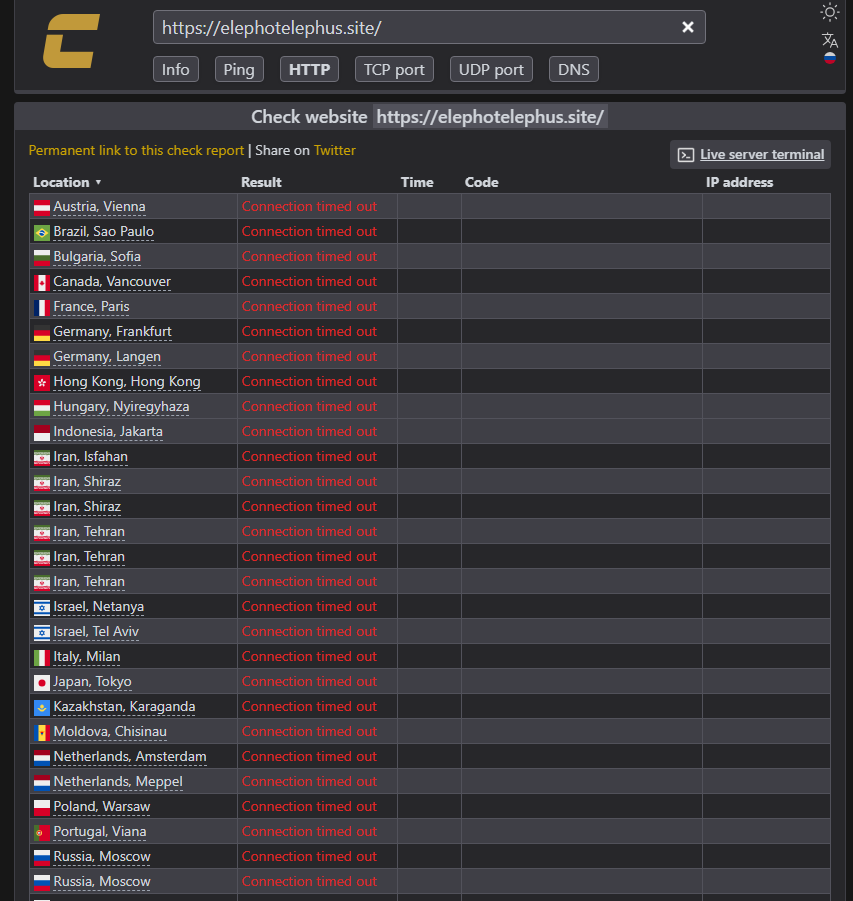
\includegraphics[width=0.78\linewidth,height=0.42\textheight,keepaspectratio]{figures/check-host.png}
\caption*{\textbf{ภาพที่ 6.1} ทดสอบเข้าเว็บไซต์จากเครื่องในหลายประเทศด้วย check-host.net ทุกจุดหมดเวลา (Connection timed out)}
\end{figure}

\begin{figure}[!htbp]
\centering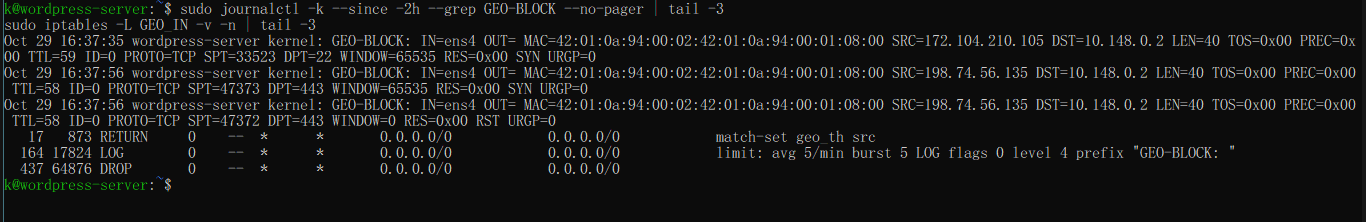
\includegraphics[width=1.00\linewidth,height=0.42\textheight,keepaspectratio]{figures/geo-block-log.png}
\caption*{\textbf{ภาพที่ 6.2} log GEO-BLOCK ของ IP ต่างประเทศที่พยายามต่อพอร์ต 22 และ 443 และตัวนับของ chain GEO\_IN}
\end{figure}

\section*{6.2 การโจมตีที่ตรวจพบจริง}\addcontentsline{toc}{section}{6.2 การโจมตีที่ตรวจพบจริง}

ข้อมูลจาก dashboard เมื่อวันที่ 29 ตุลาคม 2569 ทุกตัวเลขมาจาก log จริงของเซิร์ฟเวอร์ ไม่มีข้อมูลจำลอง

\begin{figure}[!htbp]
\centering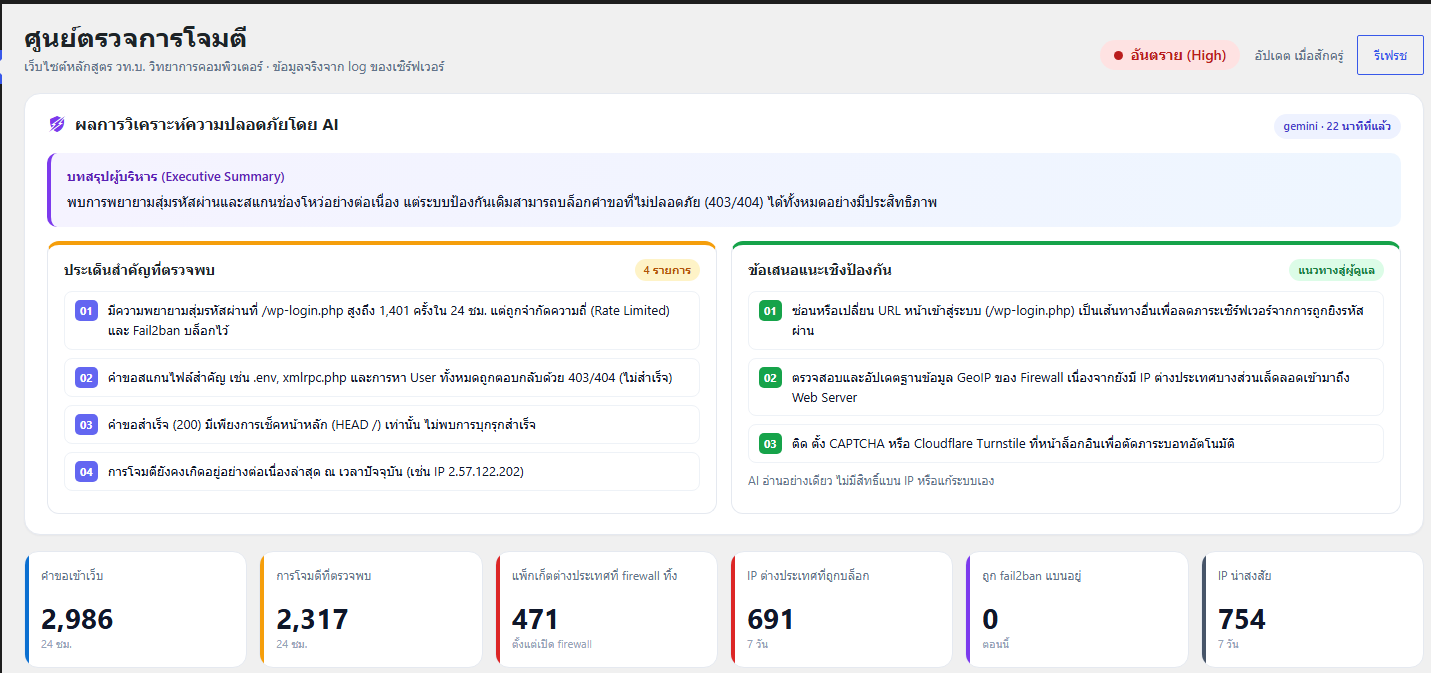
\includegraphics[width=1.00\linewidth,height=0.42\textheight,keepaspectratio]{figures/dashboard-ai.png}
\caption*{\textbf{ภาพที่ 6.3} กล่องสรุปจาก AI (Gemini) และตัวเลขหลักของ dashboard}
\end{figure}

\begingroup\small\begin{longtable}[]{@{}>{\raggedright\arraybackslash}p{0.485\linewidth - 2\tabcolsep}>{\raggedright\arraybackslash}p{0.485\linewidth - 2\tabcolsep}@{}}
\toprule\noalign{}
ตัวชี้วัด & ค่า \\
\midrule\noalign{}
\endhead
\bottomrule\noalign{}
\endlastfoot
คำขอเข้าเว็บ (24 ชม.) & 2,986 ครั้ง \\
การโจมตีที่ตรวจพบ (24 ชม.) & 2,317 เหตุการณ์ \\
SSH เข้าไม่สำเร็จ (24 ชม.) & 212 ครั้ง (ไม่มีครั้งใดสำเร็จ เพราะใช้กุญแจเท่านั้น) \\
/wp-login.php ถูกโจมตี (7 วัน) & 2,734 ครั้ง \\
IP ต่างประเทศที่ถูกบล็อก (7 วัน) & 691 IP \\
แพ็กเก็ตต่างประเทศที่ firewall ทิ้ง (ตั้งแต่เปิดใหม่) & 471 แพ็กเก็ต \\
ผลลัพธ์ HTTP (24 ชม.) & 2xx 2,280 · 3xx 130 · 4xx 577 · 5xx 0 \\
\end{longtable}\endgroup

\begin{figure}[!htbp]
\centering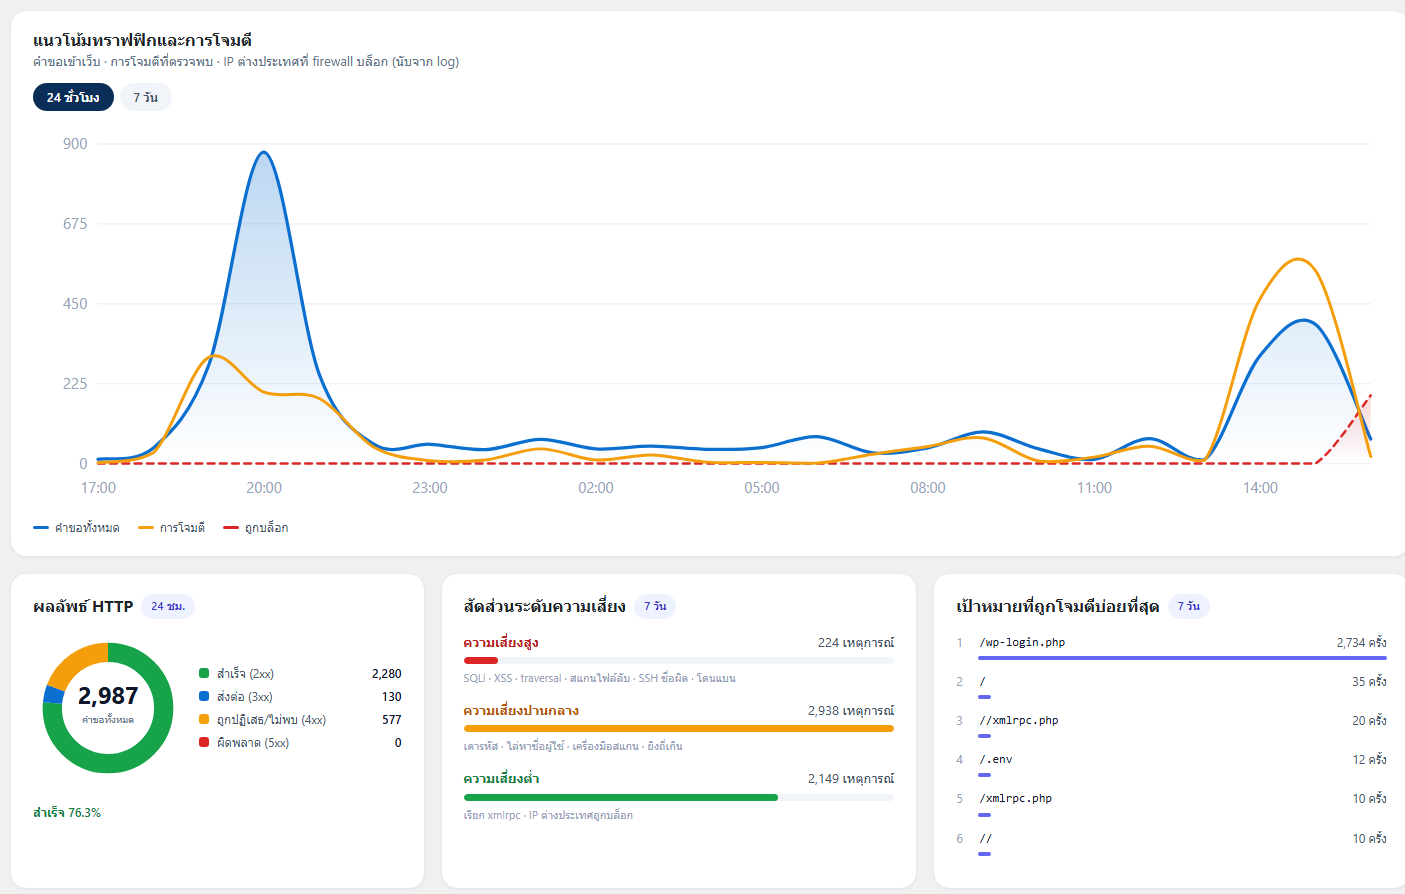
\includegraphics[width=1.00\linewidth,height=0.42\textheight,keepaspectratio]{figures/dashboard-chart.png}
\caption*{\textbf{ภาพที่ 6.4} กราฟ 24 ชั่วโมง สัดส่วนผลลัพธ์ HTTP ระดับความเสี่ยง และ URL ที่ถูกโจมตีบ่อยที่สุด}
\end{figure}

สิ่งที่พบ

\begin{itemize}
\tightlist
\item
  การโจมตีส่วนใหญ่เป็นการเดารหัสผ่านที่ /wp-login.php IP อันดับหนึ่งคือ 64.227.79.185 (ต่างประเทศ) 1,004 เหตุการณ์ ทุกครั้งถูก rate limit (429) และไม่มีครั้งใดเข้าระบบได้
\item
  IP 92.118.39.77 พยายามเข้า SSH ด้วยชื่อผู้ใช้ที่ไม่มีอยู่ และถูก fail2ban แบนอัตโนมัติ
\item
  คำขอไฟล์ลับ (.env) และ xmlrpc.php ถูกปฏิเสธทุกครั้ง
\item
  ไม่มีข้อผิดพลาด 5xx เลย เซิร์ฟเวอร์ให้บริการได้ปกติแม้ถูกโจมตีต่อเนื่อง
\end{itemize}

\begin{figure}[!htbp]
\centering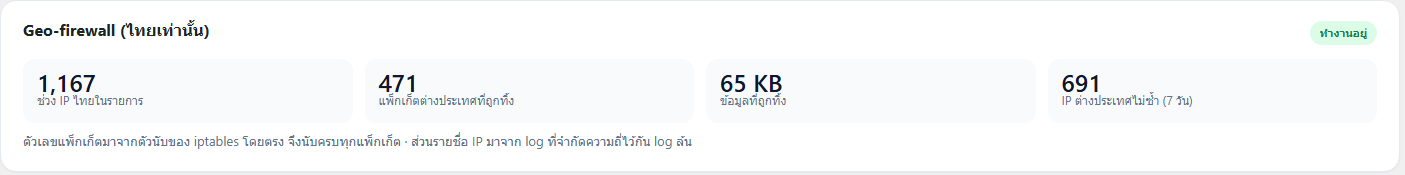
\includegraphics[width=1.00\linewidth,height=0.42\textheight,keepaspectratio]{figures/dashboard-firewall.png}
\caption*{\textbf{ภาพที่ 6.5} การ์ด Geo-firewall: ช่วง IP ไทย 1,167 ช่วง และตัวนับแพ็กเก็ตที่ถูกทิ้งจาก iptables}
\end{figure}

\begin{figure}[!htbp]
\centering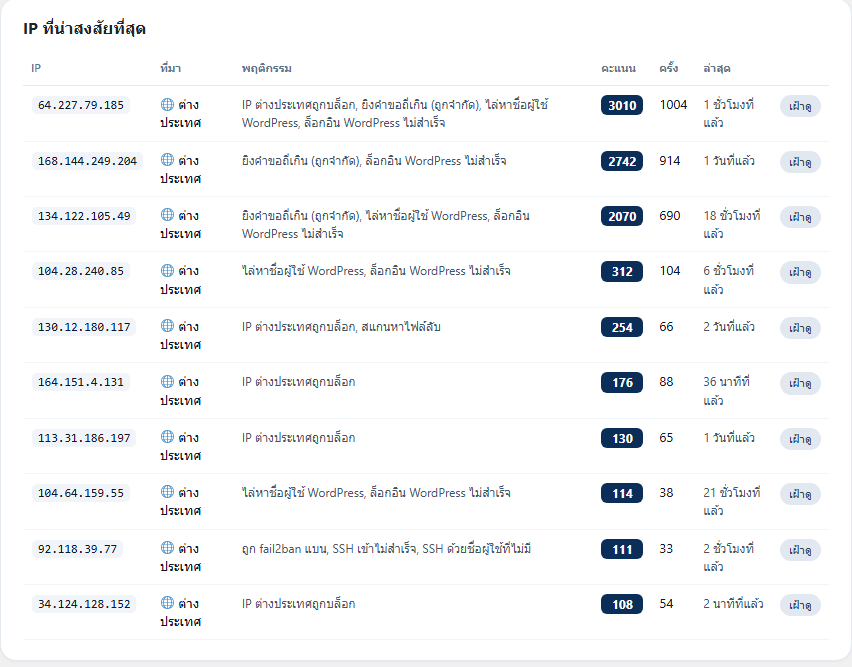
\includegraphics[width=0.77\linewidth,height=0.42\textheight,keepaspectratio]{figures/dashboard-top-ip.png}
\caption*{\textbf{ภาพที่ 6.6} IP ที่น่าสงสัยที่สุด จัดอันดับตามคะแนนความเสี่ยง}
\end{figure}

ข้อสังเกตสำคัญ: ช่วงวันที่ 28--29 ตุลาคม geo-firewall ปิดอยู่ชั่วคราว เพราะผู้ดูแลสั่ง apply ใหม่แต่ไม่ได้ยืนยันภายใน 3 นาที ระบบจึงย้อนกลับเองตามที่ออกแบบไว้ ในช่วงนั้นกราฟแสดงคำขอและการโจมตีพุ่งสูงทันที (ช่วง 20:00 และ 14:00--16:00) เมื่อเปิด firewall กลับมา เส้น ``ถูกบล็อก'' จึงเพิ่มขึ้นแทน เหตุการณ์นี้แสดงให้เห็นทั้งความสำคัญของ firewall และประโยชน์ของการป้องกันหลายชั้น เพราะระหว่างที่ firewall ปิด rate limit, fail2ban และ SSH แบบกุญแจยังกันการบุกรุกไว้ได้ทั้งหมด

นอกจากนี้ในตาราง IP พบ 34.124.128.152 ซึ่งเป็น IP ของเซิร์ฟเวอร์เอง ถูกนับเป็น IP ต่างประเทศ เกิดจาก WordPress เรียกตัวเองผ่านโดเมน (WP-Cron) แล้วถูก geo-firewall บล็อก คณะผู้จัดทำแก้โดยให้ geo-firewall อนุญาต IP ของเซิร์ฟเวอร์เองโดยอัตโนมัติ (ดูบทที่ 7)

\section*{6.3 การตรวจสอบคำแนะนำของ AI}\addcontentsline{toc}{section}{6.3 การตรวจสอบคำแนะนำของ AI}

AI สรุปว่า ``พบการสแกนหาไฟล์ตั้งค่าความลับตระกูล .env และการค้นหาชื่อผู้ใช้ WordPress จาก IP ต่างประเทศอย่างต่อเนื่อง'' คณะผู้จัดทำนำคำแนะนำมาตรวจกับระบบจริงก่อนนำไปใช้

\begingroup\small\begin{longtable}[]{@{}>{\raggedright\arraybackslash}p{0.425\linewidth - 2\tabcolsep}>{\raggedright\arraybackslash}p{0.545\linewidth - 2\tabcolsep}@{}}
\toprule\noalign{}
คำแนะนำของ AI & ผลการตรวจ \\
\midrule\noalign{}
\endhead
\bottomrule\noalign{}
\endlastfoot
ตั้งค่าเว็บเซิร์ฟเวอร์ให้ปฏิเสธไฟล์ .env & ทำไว้แล้วตั้งแต่ติดตั้ง (location \textasciitilde{} /.) \\
บล็อก IP ที่สแกน และพิจารณา GeoIP blocking & มี geo-firewall และ fail2ban อยู่แล้ว คำแนะนำนี้เกิดจาก AI ไม่ทราบบริบท \\
ปิดการไล่หาชื่อผู้ใช้และจำกัด REST API & ถูกต้อง ยังไม่ได้ปิด เป็นงานที่ควรทำต่อ (บทที่ 7) \\
\end{longtable}\endgroup

คณะผู้จัดทำจึงปรับให้สคริปต์ส่งรายการมาตรการที่มีอยู่ และ status code ของแต่ละคำขอให้ AI ด้วย ผลคือ AI ต้องใช้ควบคู่กับการตัดสินใจของคน ไม่ควรเชื่อตามทุกข้อ

\chapter*{บทที่ 7 สรุป ปัญหา และข้อเสนอแนะ}\addcontentsline{toc}{chapter}{บทที่ 7 สรุป ปัญหา และข้อเสนอแนะ}

\section*{7.1 สรุปผล}\addcontentsline{toc}{section}{7.1 สรุปผล}

คณะผู้จัดทำติดตั้ง WordPress บนเซิร์ฟเวอร์คลาวด์ด้วยตนเองครบทั้ง 3 ขั้นตามโจทย์ เว็บไซต์เข้าถึงได้ที่ \url{https://elephotelephus.site} ผ่าน HTTPS, SSH ใช้กุญแจเท่านั้นและปิด root, geo-firewall รับเฉพาะ IP ไทย 1,167 ช่วงและบล็อกการทดสอบจากต่างประเทศได้ทั้งหมด และเว็บไซต์ประชาสัมพันธ์สาขาใช้งานได้จริงพร้อมข่าวจากคณะที่อัปเดตเอง

ส่วนเพิ่มเติมคือระบบ secdash ที่ทำให้เห็นการโจมตีที่เกิดขึ้นจริง เช่น บอทสแกนไฟล์ลับและการไล่หาชื่อผู้ใช้ และใช้ AI สรุปเป็นภาษาไทยทุกชั่วโมง บทเรียนสำคัญคือการป้องกันหลายชั้นทำให้ชั้นหนึ่งที่พลาดไม่กลายเป็นความเสียหาย และคำแนะนำจาก AI ต้องตรวจกับระบบจริงก่อนนำไปใช้

\section*{7.2 ปัญหาและแนวทางแก้ไข}\addcontentsline{toc}{section}{7.2 ปัญหาและแนวทางแก้ไข}

ตารางที่ 7.1 ปัญหาที่พบระหว่างทำโครงงาน

\begin{longtable}[]{@{}>{\raggedright\arraybackslash}p{0.242\linewidth - 2\tabcolsep}>{\raggedright\arraybackslash}p{0.364\linewidth - 2\tabcolsep}>{\raggedright\arraybackslash}p{0.364\linewidth - 2\tabcolsep}@{}}
\toprule\noalign{}
ปัญหา & สาเหตุ & วิธีแก้ \\
\midrule\noalign{}
\endhead
\bottomrule\noalign{}
\endlastfoot
setup.sh หยุดทำงานเงียบๆ หลังใส่ Zone ID & ฟังก์ชันสุ่มรหัสผ่านใช้ pipe ที่เกิด SIGPIPE เมื่อเปิด set -e & อ่านจาก /dev/urandom เป็นก้อนขนาดคงที่แทน และตรวจ token กับ Cloudflare ก่อนทำต่อ \\
ตั้งค่าภาษา WordPress ไม่สำเร็จ & ไม่พบไฟล์ภาษา th ในขั้นติดตั้ง & ติดตั้งเป็น en\_US แล้วเปลี่ยนภาษาภายหลังในหน้าตั้งค่า \\
wp-cli สร้าง rewrite rule ไม่ได้ & สิทธิ์ไดเรกทอรีทำงานไม่ตรงกับผู้ใช้ www-data & เรียก wp-cli เป็น www-data ในโฟลเดอร์เว็บ และไม่ใช้ -\/-hard \\
เว็บตอบ NXDOMAIN & มี A record เฉพาะ cs ยังไม่มี @ & เพิ่ม A record ของ @ และล้าง DNS cache \\
แหล่ง IP ไทย (ipdeny) ส่งรายการว่าง & ดาวน์โหลดไม่สำเร็จ สคริปต์จึงไม่ยอมเปิด firewall & เปลี่ยนไปใช้ไฟล์สถิติของ APNIC และเก็บ ipdeny เป็นแหล่งสำรอง \\
สคริปต์หา IP ของผู้ดูแลไม่เจอ & sudo ลบตัวแปร SSH\_CLIENT & ใช้ค่าสำรองจาก who -m \\
ขั้น 2FA ถูกนับเป็น login ผิด & หน้า 2FA ตอบ 200 เหมือนรหัสผิด & ตัดออกเมื่อ 2FA สำเร็จตามมาใน 5 นาที \\
IP ของทีมถูกนับเป็นผู้โจมตี & ตัวแก้ไขบทความเรียก API รายชื่อผู้ใช้ & IP ที่ login สำเร็จถือเป็นคนในทีม \\
เรียก AI ไม่สำเร็จ (404, 503, timeout) & โมเดลเดิมถูกปลด เซิร์ฟเวอร์ AI ไม่ว่าง และรุ่นใหม่ตอบช้า & เลือกรุ่นอัตโนมัติ รอนานขึ้น และสลับรุ่นเมื่อมีปัญหา \\
DBeaver ต่อฐานข้อมูลไม่ได้ & ตั้งให้ต่อตรงพอร์ต 3306 ซึ่งไม่ได้เปิด & ใช้ SSH tunnel และตั้ง allowPublicKeyRetrieval \\
\end{longtable}

\section*{7.3 ข้อจำกัด}\addcontentsline{toc}{section}{7.3 ข้อจำกัด}

\begin{itemize}
\tightlist
\item
  geo-firewall กันผู้โจมตีที่ใช้ IP ไทย (VPN ไทย หรือเครื่องในไทย) ไม่ได้ จึงต้องพึ่งชั้นอื่นด้วย
\item
  คนไทยที่อยู่ต่างประเทศและบริการตรวจเว็บจากต่างประเทศ (เช่น SSL Labs) เข้าเว็บไม่ได้
\item
  การจัดประเภทการโจมตีใช้รูปแบบที่กำหนดไว้ การโจมตีแบบใหม่อาจไม่ถูกตรวจพบ
\item
  เซิร์ฟเวอร์มีเครื่องเดียว ถ้าเครื่องล่มเว็บจะหยุดให้บริการ
\end{itemize}

\section*{7.4 ข้อเสนอแนะ}\addcontentsline{toc}{section}{7.4 ข้อเสนอแนะ}

\begin{enumerate}
\def\labelenumi{\arabic{enumi}.}
\tightlist
\item
  ติดตามแพตช์ถาวรของ CVE-2026-115560 แล้วอัปเดต PHP ทันทีที่ออก และรัน security-check.sh เป็นประจำ
\item
  ใช้ reverse proxy หรือ cache ของ Cloudflare เพื่อเพิ่มความเร็วและซ่อน IP จริง โดยย้ายการกรองประเทศไปไว้ที่ Cloudflare
\item
  ส่งแจ้งเตือนทันที (เช่น อีเมลหรือ LINE) เมื่อระดับความเสี่ยงเป็น ``สูง''
\item
  เก็บไฟล์สำรองไว้นอกเซิร์ฟเวอร์ เช่น Cloud Storage กันกรณีเครื่องเสียหายทั้งเครื่อง
\item
  เพิ่ม Web Application Firewall เช่น ModSecurity กับชุดกฎ OWASP CRS
\end{enumerate}

\chapter*{บรรณานุกรม}\addcontentsline{toc}{chapter}{บรรณานุกรม}

ทุกรายการสืบค้นเมื่อ 27 ตุลาคม 2569

\begin{enumerate}
\def\labelenumi{\arabic{enumi}.}
\tightlist
\item
  APNIC. (n.d.). \emph{APNIC delegated statistics}. จาก \url{https://ftp.apnic.net/stats/apnic/}
\item
  Barnes, R., Hoffman-Andrews, J., McCarney, D., \& Kasten, J. (2019). \emph{RFC 8555: Automatic Certificate Management Environment (ACME)}. จาก \url{https://www.rfc-editor.org/rfc/rfc8555}
\item
  Cloudflare. (n.d.). \emph{Cloudflare DNS documentation}. จาก \url{https://developers.cloudflare.com/dns/}
\item
  fail2ban. (n.d.). \emph{fail2ban}. จาก \url{https://github.com/fail2ban/fail2ban}
\item
  Google. (n.d.). \emph{Compute Engine documentation}. จาก \url{https://cloud.google.com/compute/docs}
\item
  Google. (n.d.). \emph{Gemini API documentation}. จาก \url{https://ai.google.dev/gemini-api/docs}
\item
  Internet Security Research Group. (n.d.). \emph{Challenge types}. Let's Encrypt. จาก \url{https://letsencrypt.org/docs/challenge-types/}
\item
  acme.sh. (n.d.). \emph{acme.sh: A pure Unix shell script implementing ACME client protocol}. จาก \url{https://github.com/acmesh-official/acme.sh}
\item
  Netfilter Project. (n.d.). \emph{ipset}. จาก \url{https://ipset.netfilter.org/}
\item
  Netfilter Project. (n.d.). \emph{The netfilter.org project}. จาก \url{https://www.netfilter.org/}
\item
  nginx. (n.d.). \emph{nginx documentation}. จาก \url{https://nginx.org/en/docs/}
\item
  Oracle. (n.d.). \emph{MySQL 8.0 Reference Manual}. จาก \url{https://dev.mysql.com/doc/refman/8.0/en/}
\item
  OWASP Foundation. (n.d.). \emph{OWASP Top Ten}. จาก \url{https://owasp.org/www-project-top-ten/}
\item
  The PHP Group. (n.d.). \emph{FastCGI Process Manager (FPM)}. จาก \url{https://www.php.net/manual/en/install.fpm.php}
\item
  Ubuntu. (n.d.). \emph{sshd\_config(5)}. จาก \url{https://manpages.ubuntu.com/manpages/noble/man5/sshd_config.5.html}
\item
  WordPress.org. (n.d.). \emph{Hardening WordPress}. จาก \url{https://developer.wordpress.org/advanced-administration/security/hardening/}
\item
  WordPress.org. (n.d.). \emph{REST API Handbook}. จาก \url{https://developer.wordpress.org/rest-api/}
\item
  WordPress.org. (n.d.). \emph{Two-Factor plugin}. จาก \url{https://wordpress.org/plugins/two-factor/}
\item
  Ylonen, T., \& Lonvick, C. (2006). \emph{RFC 4252: The Secure Shell (SSH) Authentication Protocol}. จาก \url{https://www.rfc-editor.org/rfc/rfc4252}
\end{enumerate}

\thaichapter{}{ภาคผนวก}\addcontentsline{toc}{chapter}{ภาคผนวก}

\section*{ภาคผนวก ก คำสั่งตรวจสอบระบบ}\addcontentsline{toc}{section}{ภาคผนวก ก คำสั่งตรวจสอบระบบ}

คำสั่งเหล่านี้ใช้เก็บหลักฐานในบทที่ 6 และใช้สาธิตต่ออาจารย์ได้

\begin{Verbatim}[breaklines,breakanywhere,fontsize=\small,frame=single,framesep=6pt]
# ขั้น 1: SSH
sudo sshd -T | grep -Ei 'permitrootlogin|passwordauthentication|authenticationmethods'
ssh root@34.124.128.152            # ต้องได้ Permission denied
last -n 20                          # ประวัติการเข้าเครื่อง

# ขั้น 1: เวอร์ชันและบริการ
sudo cat /root/versions.txt
sudo fail2ban-client status
sudo ss -ltnp | grep 3306           # ต้องเป็น 127.0.0.1:3306

# ขั้น 2: firewall
sudo bash geo-firewall.sh status
sudo journalctl -k --since -1d --grep GEO-BLOCK | tail

# ส่วนเพิ่ม: secdash
sudo python3 /usr/local/sbin/secdash-collect.py
\end{Verbatim}

\section*{ภาคผนวก ข ดัชนีภาพหน้าจอ}\addcontentsline{toc}{section}{ภาคผนวก ข ดัชนีภาพหน้าจอ}

\begingroup\small\begin{longtable}[]{@{}>{\raggedright\arraybackslash}p{0.651\linewidth - 2\tabcolsep}>{\raggedright\arraybackslash}p{0.319\linewidth - 2\tabcolsep}@{}}
\toprule\noalign{}
หลักฐาน & ภาพ \\
\midrule\noalign{}
\endhead
\bottomrule\noalign{}
\endlastfoot
แผนภาพสถาปัตยกรรม และ versions.txt & ภาพที่ 3.1--3.2 \\
HTTPS ใน Chrome (ใบรับรองถูกต้อง, TLS 1.3) & ภาพที่ 4.1 \\
SSH: sshd -T และ root ถูกปฏิเสธ & ภาพที่ 4.2--4.3 \\
fail2ban 3 jail & ภาพที่ 4.4 \\
geo-firewall status และ log GEO-BLOCK & ภาพที่ 4.5, 6.2 \\
หน้าแรกบนคอมพิวเตอร์และมือถือ & ภาพที่ 4.6--4.7 \\
Customizer, DBeaver ผ่าน SSH tunnel, หน้าข่าวสาร & ภาพที่ 4.8--4.10 \\
security-check: แพตช์ PHP, checksum, ผลสรุป FAIL 0 & ภาพที่ 4.11--4.13 \\
check-host.net: ต่างประเทศเข้าไม่ได้ & ภาพที่ 6.1 \\
dashboard ตรวจการโจมตีและ AI & ภาพที่ 6.3--6.6 \\
\end{longtable}\endgroup

\section*{ภาคผนวก ค รายการไฟล์ที่พัฒนา}\addcontentsline{toc}{section}{ภาคผนวก ค รายการไฟล์ที่พัฒนา}

\begingroup\small\begin{longtable}[]{@{}>{\raggedright\arraybackslash}p{0.485\linewidth - 2\tabcolsep}>{\raggedright\arraybackslash}p{0.485\linewidth - 2\tabcolsep}@{}}
\toprule\noalign{}
ไฟล์ & หน้าที่ \\
\midrule\noalign{}
\endhead
\bottomrule\noalign{}
\endlastfoot
setup.sh & ติดตั้งและตั้งค่าเซิร์ฟเวอร์ทั้งหมด (SSH, LEMP, WordPress, HTTPS, fail2ban, สำรองข้อมูล) \\
geo-firewall.sh & firewall รับเฉพาะ IP ไทย (apply, confirm, status, update, off) \\
secdash/secdash-collect.py & อ่าน log จัดประเภทการโจมตี เรียก AI และเขียน summary.json \\
secdash/secdash-install.sh & ติดตั้งตัวเก็บข้อมูลและ cron \\
ธีม buu-informatics: functions.php, front-page.php, header.php, footer.php & โครงสร้างและหน้าต่างๆ ของเว็บไซต์ \\
inc/content.php & ค่าตั้งเนื้อหาที่แก้ได้ใน Customizer และการดึงข่าว \\
inc/import.php & นำเข้าข่าวคณะเป็นโพสต์ WordPress \\
inc/secdash.php & หน้า dashboard ``ความปลอดภัย'' ในหลังบ้าน \\
\end{longtable}\endgroup


\end{document}
